\chapter{\texorpdfstring{$\Ca$ channel models}{Ca2+ Channel Models}}
\label{chap:dhpr-models}
\label{chap:Ca-channel-models}

In the chapter~\ref{chap:kinetics-channels}, we have learnt how the models for
ion channels, particularly focusing on Markov models, are developed from
experimental data. In this chapter, we will discover in detail models for $\Ca$
channels (Chap.\ref{chap:VDCC_Intro}), specifically L-type $\Ca$ channels (aka
Dihydropyridine Receptors (DHPR)).
Other types of ion channels will be discussed in the coming chapters.

The gating of LCCs is believed to be voltage-dependent. However, the
inactivation is more complex, and is thought both voltage- and [Ca]-dependent.
We will discuss in detail in Sect.~\ref{sec:LCC_activation_inactivation}.

 
\begin{table}[hbt]
\begin{center}
\begin{tabular}{p{4cm}|p{3.0cm}p{4cm}}
%\begin{tabular}{l|l|l}
\hline \\ 
& T-type & L-type \\
\hline \\
voltage activation threshold & -60 to -50 mV (in SA) & -40 mV (in SA) \\
	& -50 mV (atria, not human) & -30 mV (atria) \\
	conductance (pS) & 8 & 25 \\
	mean open time (ms) & 1-2 & $< 1$ \\
	inactivation kinetics & fast & slow \\
	Bay K 8644 & no effect & open channel \\
	$\beta$-receptor  stimulation & no effect & major effect \\
	blocker & nickel, amiloride, mibefradil & verapamil, nifedipine diltiazem, D600 (2$\muM$)\\
	\hline
\end{tabular}
\caption{Properties of T-type vs. L-type \citep{opie2004}}
\end{center}
\end{table}

\section{New papers}

\citep{schroder1998, findlay2002, peterson1999}


\section{Introduction}
\label{sec:introduction-10}

There are two types of calcium channels that can contribute to pacemaker
activity, AP upstroke \& plateau phases, and arrhythmias [particularly {\it
tachycardia} - {\it early afterdepolarisation} (EAD)]. They are L-type
($I_{Ca,L}$ - Sect.\ref{sec:L-type-Ca2+}) and T-type ($I_{Ca,T}$
- Sect.\ref{sec:T-type-Ca2+})~\citep{bers2008cca}.

Another name for L-type $\Ca$ channel is DHPR (Sect.\ref{sec:DHPR-Ca2+channel}).
DHPR, in cardiac muscle, whose number varies from 10-100\% of the
number of RyR2s, are localized at the diad junctions, but are randomly
positioned relative to the RyR lattice. \textcolor{red}{This contrasts
to the regular arrangement of DHPR tetrads found in skeletal
muscle}. 


\subsection{Effect of blockers (antagonists)}

These are well-known blockers of $I_\CaL$ (review: \citep{janis1983, janis1984}) 
\begin{enumerate}
  \item Phenylalkylamines (e.g. verapamil, D600): relatively selective for
  myocardium
  \item dihydropyridine (DHPR), e.g. nitrendipine, difedipine
  \item $\Ca$-calmodulin inhibitor, e.g. fendiline
\end{enumerate}
Some can have dual effects on LCC, e.g. DHPR can provoke a small transient
stimulation prior to inhibition \citep{hess1984, brown1984, brown1985} or D600
\citep{mcdonald1989}.

Nonselective: These blockers have blocking effect on all $\Ca$ channels
\begin{enumerate}
  \item Mibefradil (Posicor): a drug used for treatment of hypertension
  \item  bepridil
  \item fendiline
\end{enumerate}

\url{https://en.wikipedia.org/wiki/Calcium_channel_blocker}

\subsection{Effect of agonists}
\label{sec:DHPR_agonists}

Agonists: Bay K 8644 (-), benzoyl pyrrole FPL 64176, CGP 28 392.

\begin{framed}
There are 2 types of Bay K 8644:
\begin{enumerate}
\item (+) isomer: an LCC antagonist
\item (-) isomer: an LCC agonist
\end{enumerate}
It's the membrane potential that determine whether Bay K 8644 acts as an agonist
or antagonist \citep{Sanguinetti1986}. There are other factors that affect the
antagonism of Bay K 8644 to L-type $\Ca$ channels.
\end{framed}
  
Bay K 8644 (-) and benzoyl pyrrole FPL 64176 both shift the
$V_m$-dependent activation/inactivation to a more negative value (i.e. -10mV).
Besides, FPL 64176 show the rate of activation and decline of $\Ca$ current,
while Bay K 8644 accelerate the rate of current decay~\citep{fan2000}. Bay K
8644 (-) and CGP 28 392 enhance macroscopic currents by prolong the mean open
time \citep{hess1984, kokubun1984}. 

% \subsubsection{Bay K 8644 (-)}
% \label{sec:bay-k-8644}

As it's not easy to measure single channel current, to enhance the LCC current,
they prolong the LCC opening by using Bay K 8644 (-). At [Bay K 8644] = 1$\mu$M,
LCC currents reach the maximum, i.e. 3-fold and the $V_{1/2}$ of the activation
curve of LCC is shifted from -10 to -17.5 mV in the I-V
curve~\citep{january1988}. To account for this change:
\begin{enumerate}
\item In addition, the activation time constant $\tau_d$, at all
  potentials, is reduced by 11\%.

\item A 10mV shift is introduced in the negative direction of
  steady-state inactivation curve $f_\infty$ and $\tau_f$ of $I_\CaL$.
\item The values of $f_\infty$ and $\tau_f$ is reduced by 5\% to
  reflect the acceleration of inactivation of $I_\CaL$ in the presence
  of Bay K 8644. 
\end{enumerate}

Studies first using Bay K 8644 were Sect.\ref{sec:LCC_Hess1984}. FPL 64176 exerts
its effects on by binding to a site on the pore-forming $\alpha_1$ subunit of
LCC. This site is closed to dihydropyridine binding site \citep{rampe1991}. It
causes a longer-lasting tail current than do dihydropyridine agonists, thus more
effectively isolating LCC from other neuronal $\Ca$ currents\citep{lewis1994}.
The effects of FPL 64176 on neurons has been done by \citep{Liu2003} which
shows to enhance L-type but inhibit N-type neuronal $\Ca$ channels.


\subsection{Effect of Temperature}

\citep{cavalie1985tit} used whole-cell Voltage-clamped technique to measure
I-V  curve in guinea pig ventricualr myocytes,
Fig.\ref{fig:ICaL_temperature_Cavalie1985}. The curve was unaffected when the
temperature in the range 21-37$^\circ$ C. The main affect was in the current
amplitude $I_\CaL$ and the time course. $Q_{10}$ for amplitude, time to peak,
and $T_{1/2}$ inactivation was estimated to be 2.96$\pm$0.14, 2.52$\pm$0.13, and
2.82$\pm$0.28, respectively.

\begin{figure}[hbt]
  \centerline{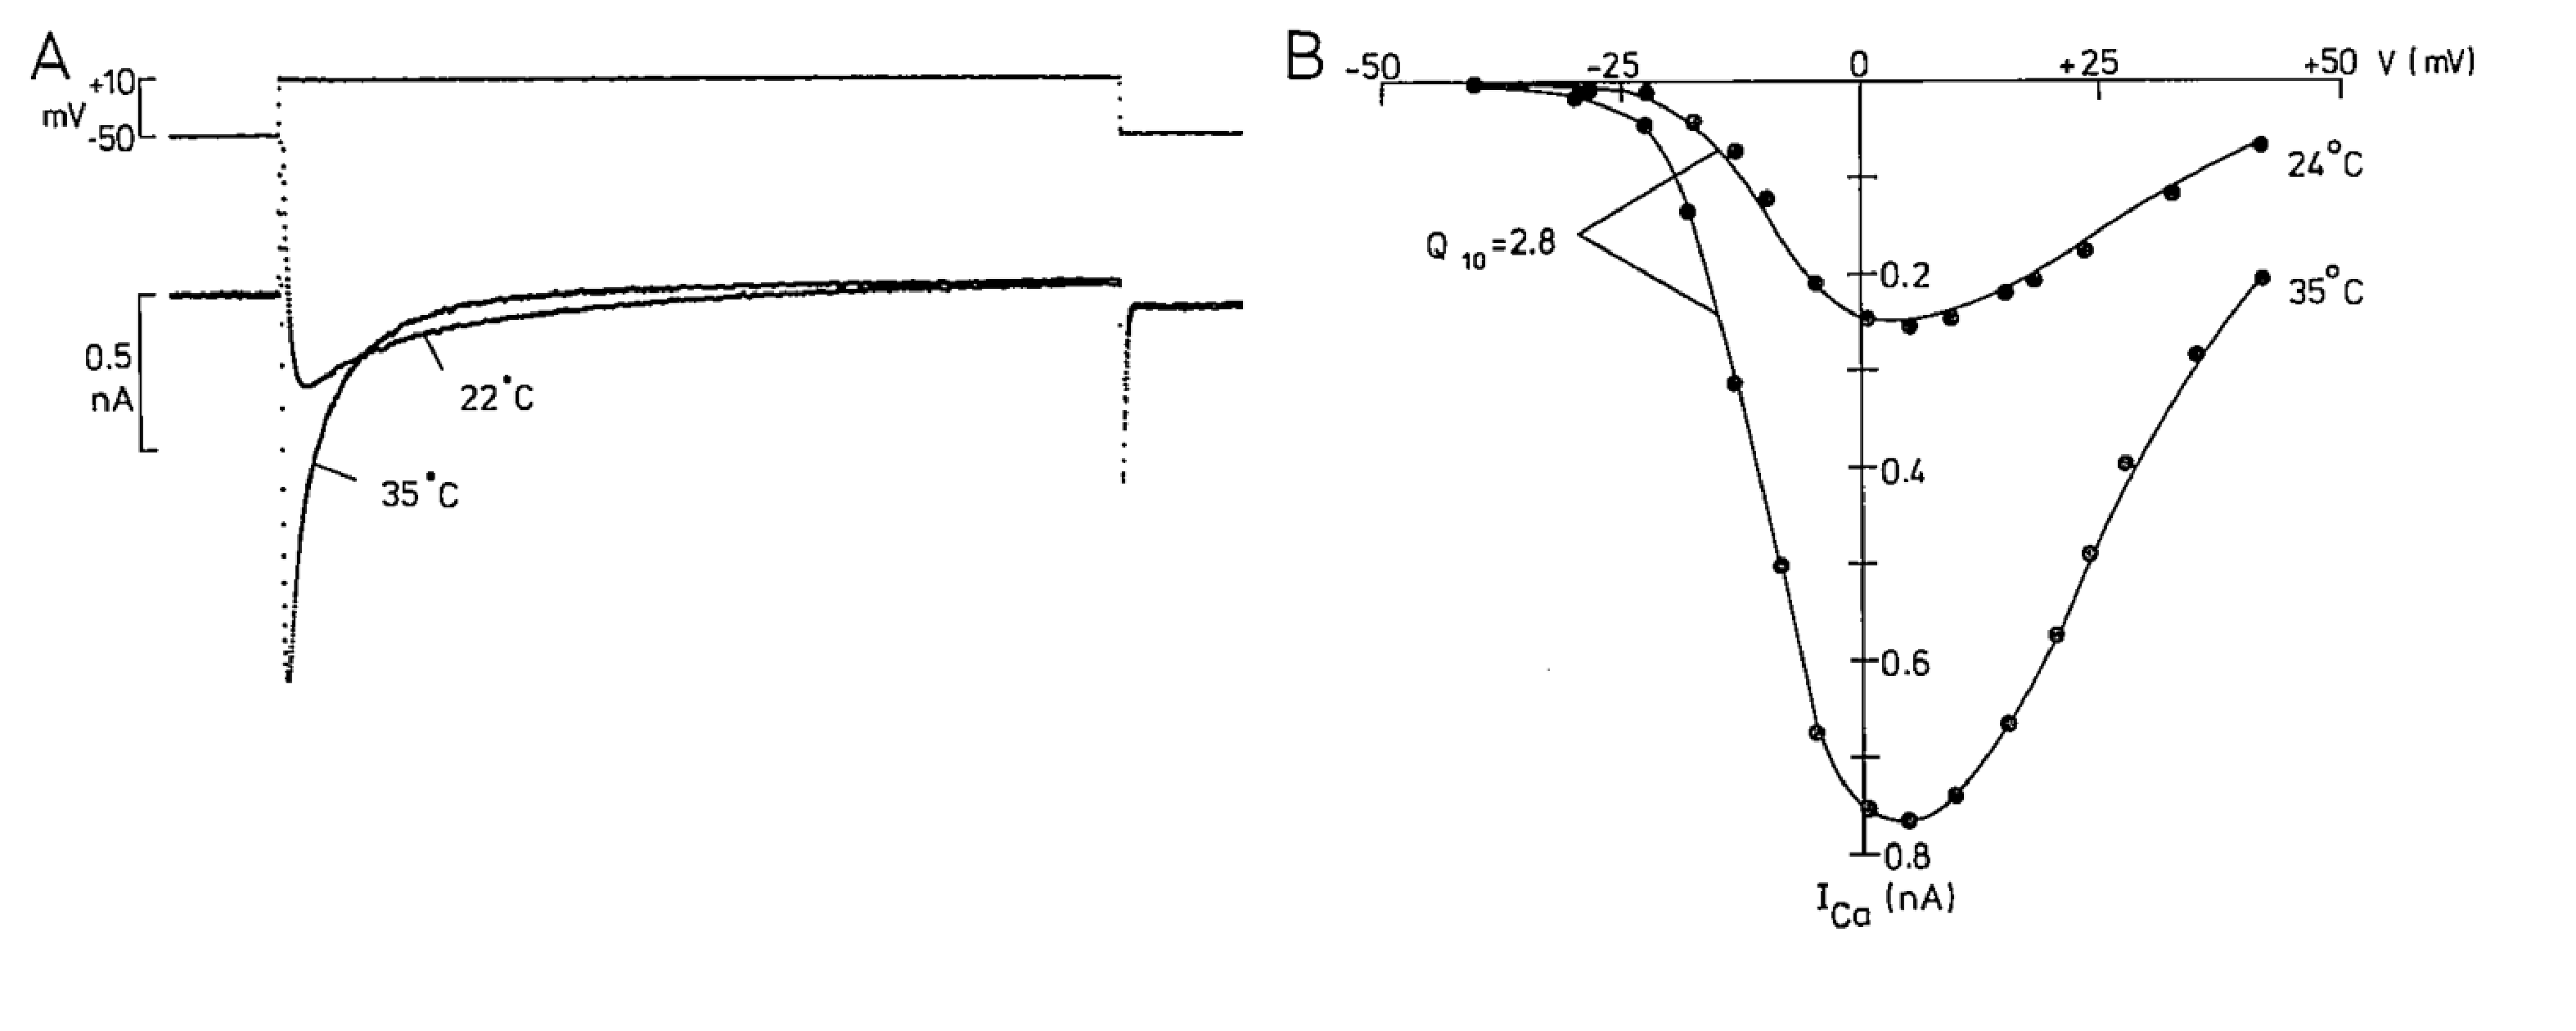
\includegraphics[height=5cm,
    angle=0]{./images/ICaL_temp_Cavalie1985.eps}}
\caption{$I_\CaL$ currents under 2 different temperatures: 22$^\circ$C and
35$^\circ$C}
\label{fig:ICaL_temperature_Cavalie1985}
\end{figure}


\subsection{Permeability and reversible potential}

$\Ca$ channels is known to permeate different ions (both monovalent and
divalent). The reversible potential $E_\rev$ was assumed
\begin{equation}
\begin{split}
E_\rev &= \frac{RT}{2F}\ln\frac{4P_\Ba a^o_\Ba}{P_\Cs a^i_\Cs + P_\Na a^i_\Na}
 \end{split}
\end{equation}
with $a^i, a^o$ represent ion activities estimated from concentrations by taking
activity coefficient $\gamma$: $\gamma_\Ba=0.26$, $\gamma_\Cs=\gamma_\Na=0.75$.
Assuming $P_\Ba/P_\Cs=1430, P_\Na/P_\Cs=3$, then $E_\rev= +94$ mV. The result
$E_\rev=+55$ mV, gave a better I-V  curve \citep{mcdonald1986}. Different
permeability gives different value for the reversable potentials. 


\subsection{Models}
\label{sec:LCC_models}

L-type $\Ca$ channels typically begin to activate between -40mV to -30mV and the
peak currents reach maximum between 0 amd +10mV. The maximal $I_\ca$ density
\begin{enumerate}
  \item rat control: 4.28$\pm$ 0.98 pA/pF \citep{delbridge1997} or in the
  presence of 1$\muM$ Isoproterenol (16.6$\pm$2.3 pA/pF)
  \item rat pressure-overload hypertrophy: 4.57$\pm$ 0.6 pA/pF
  \citep{delbridge1997}, or in the presence of 1$\muM$ Isoproterenol
  (16.5$\pm$2.3 pA/pF).
\end{enumerate}

First models of $\Ca$ channels were based on Hodgkin-Huxley formalism
(Sect.\ref{sec:difr-noble-1985}). \citep{hess1986ccs} first proposed
mode-switching model (Sect.\ref{sec:LCC_Hess1984}); then others
(Sect.\ref{sec:LCC_Imredy1994}, \ref{sec:LCC_Jafri1998}, \ref{sec:LCC_stern1999}).
Modal models can easily replicate normal gating mechanism, as well as the
effects of large depolarizations, blockage by DHPR and $\beta$-adrenergic
stimulation by simply shifting to another modes. However, mode-switching models
lead to so many states, and it's hard to fit parameters. An alternate option is
multi-state models, or Markov-chain models (Sect.\ref{sec:LCC_Sun2000}). 
In experiments, to eliminate CDI, they substitute $\Ca$ with $\Mg$ or $\Ba$. In
the Markov model, the transitions with $\Ca$-dependent inactivation are set to
zero.

To account for multi-ion permeability, and also to avoid multi-state models, GHK
equation is often used (Sect.\ref{sec:LCC_Luo1994}) with large permeability to
$\Ca$, coupled with small permeability of other ions $P_\ca/P_\na > 1000$).
However, GHK equation assume ions across the channel independently, i.e. without
interacting, while the experiment data shown that $[\Ca]_o=1$ (mM) exclude $\Na$
and $\K$, even these ions are present with a thousand times higher in
concentration \citep{mccleskey1986}. This, however, violate experimental data.

Due to the striking structural similarity in the sequence homology between $\Ca$
proteins and $\Na$ or $\K$ proteins. It's typically assumed activation is rapid
and is solely voltage dependent. However, modelling the inactivation behavior
of L-type $\Ca$ channels has long been challenging. The reason is that the
inactivation kinetics is complex with both voltage, and calcium dependence.

Experimental data shown that open probability for LCC is around 0.3 to 0.7 at
+10 to +60 (mV) depolarization \citep{cachelin1983}.

\section{Estimating channel kinetics}


A double pulse protocol is often used to measure channel currents. The cell is
kept at quiescent to steady-state (e.g. -80mV), then slowly depolarize the
channels from resting to -50 mV for 500ms. The L-type $\Ca$ channes are kept at
-50mV for 50ms, before applying different test pulses (from -40mV to +40mV with
step +10mV) \citep{santana1996}. 

In order to estimate the tail current, a ramp protocol is also used (Bargas et
al., 1994). The kinetics is then estimated using GHK formula
(Sect.\ref{sec:GHK-Ca2+}).

\subsection{Intramembrane charge movement vs. ionic currents}

In the first computational model of axon, Hodgkin-Huxley assumed the gating of
ion channels is the result of intramembrane movement of charged groups or
dipolar molecules that could change locations or orientation in reponse to
changes in $V_m$. Since then, a considerable amount of work has spent on the
role of intramembrane charge movement in serving as a voltage-sensor
\citep{Dubois1982, Schneider1973, Ahern2001}. The movement of these gating
charges in response to voltage changes can induce a substantial reorientation of
the transmembrane segments that facilitates the energetically favorable opening
of the ion-selective pore.

 Early experiments to explain how a change in transmembrane potential
across the SL and T-tubule membrane could bring about the release of $\Ca$ from the
neighobring SR showed that a movement of charges across the T-tubule

The membrane current density $i_m$ is related to the difference potential
$\Delta V = V_2 - V_1$
\begin{equation}
i_m = \frac{2 V_m}{3 r_i l^2}
\end{equation}
with $r_i$ is internal resistance per unit length of the fiber, and $l$ is the
length of the fiber. At different test pulse, from a given holding potential,
shows an 'on' and 'off' area. Also, it showed an effect of pulse duration on
charge movement \citep{Schneider1973},
Fig.\ref{fig:Vstim_Charge_movement_Schneider1973}. Here, the areas of the 'on',
and 'off' seem to match 


\begin{figure}[hbt]
  \centerline{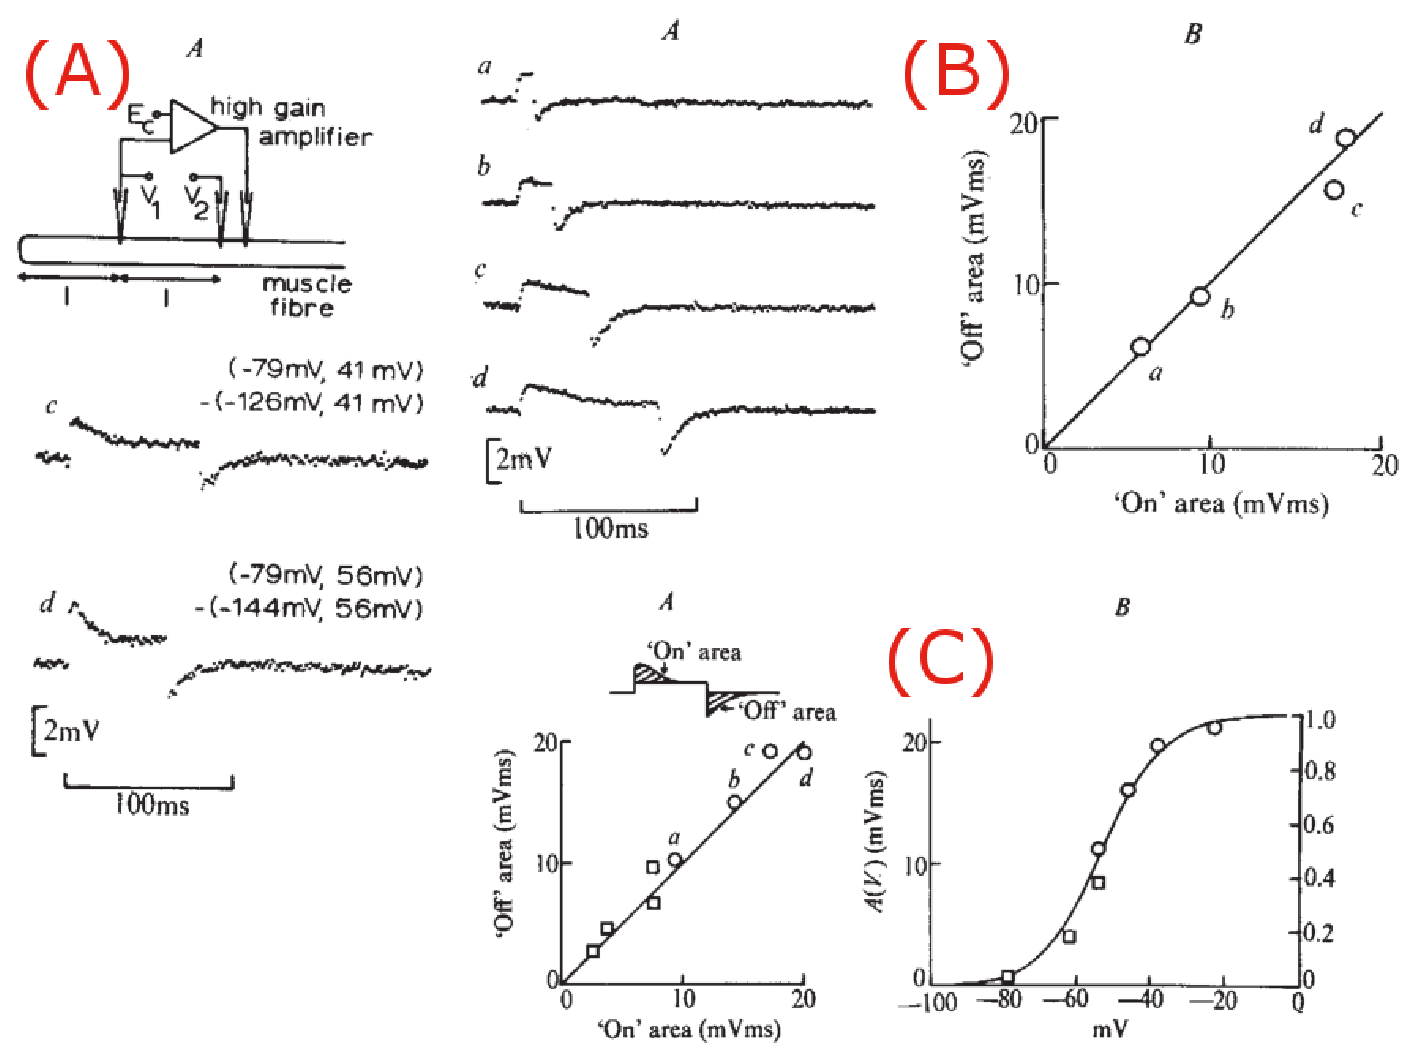
\includegraphics[height=6cm,
    angle=0]{./images/Vstim_Charge_movement_Schneider1973.eps}}
  \caption{Three microelectrode technique (holding potential -79mV, length
  $l=172\mum$). (B) Effect of pulse duration on charge movement; comparison
  between the 'on' area and 'off' area at different pulse durations. (C)
  Effect of membrane voltage on charge movement \citep{Schneider1973}}
\label{fig:Vstim_Charge_movement_Schneider1973}
\end{figure}

The goal was to investigate the relationship between charge movements and
membrane potential $V_m$. By defining the area of extra transient A(V), which
can be expressed by single exponential Boltzmann
\begin{equation}
\frac{A(V_m)}{A_\max} = \frac{1}{1+\exp(-(V-V_{1/2})/k)}
\end{equation}
with $V_{1/2}=-53$ mV, k=8 (mV), $A_\max = 22$ mV.ms,
Fig.\ref{fig:Vstim_Charge_movement_Schneider1973}(C).

The conclusion is that there is a fixed amount of charge, free to move between
different locations across the membrane or between intramembrane locations that
see different membrane potential. Here, two positions where we put two
microelectrodes $V_1$ and $V_2$. Then the potential is very negative, all the
charged groups would be in position 1; with depolarization, some will move to
position 2; on repolarization, those charged groups on position 2 would return
to 1. These movements of charge would produce transient currents resembling
those observed in the experiments aboved. If $f_1$ is the probability of the
group in position 1, $f_2$ is the probability in position 2, then the Boltzmann
expression is
\begin{equation}
\frac{f_1}{f_2} \propto \exp \left[ -\alpha z F (V-V_{1/2})/(RT) \right]
\end{equation}
with $z$ is the valence of the charge group, $V_{1/2}$ is the potential at which
$f_1=f_2$. NOTE $f_1+f_2 = 1$. NOTE $k = RT/(\alpha z F)$. Based on
\citep{Schneider1973}, the physiological role of charge movement was unknown,
yet it may has certain roles in triggering mechanisms.

To measure the real amount of charge movement $Q$, for a certain membrane
change, \citep{Adrian1976} estimated about 30nC/$\muF$ of charge moves between membrane
potential of -80 mV and 0mV, Fig.\ref{fig:charge_movement_Adrian1976}. At
membrane potential positive to 0mV, the charge movement seems to saturate.

\begin{figure}[hbt]
  \centerline{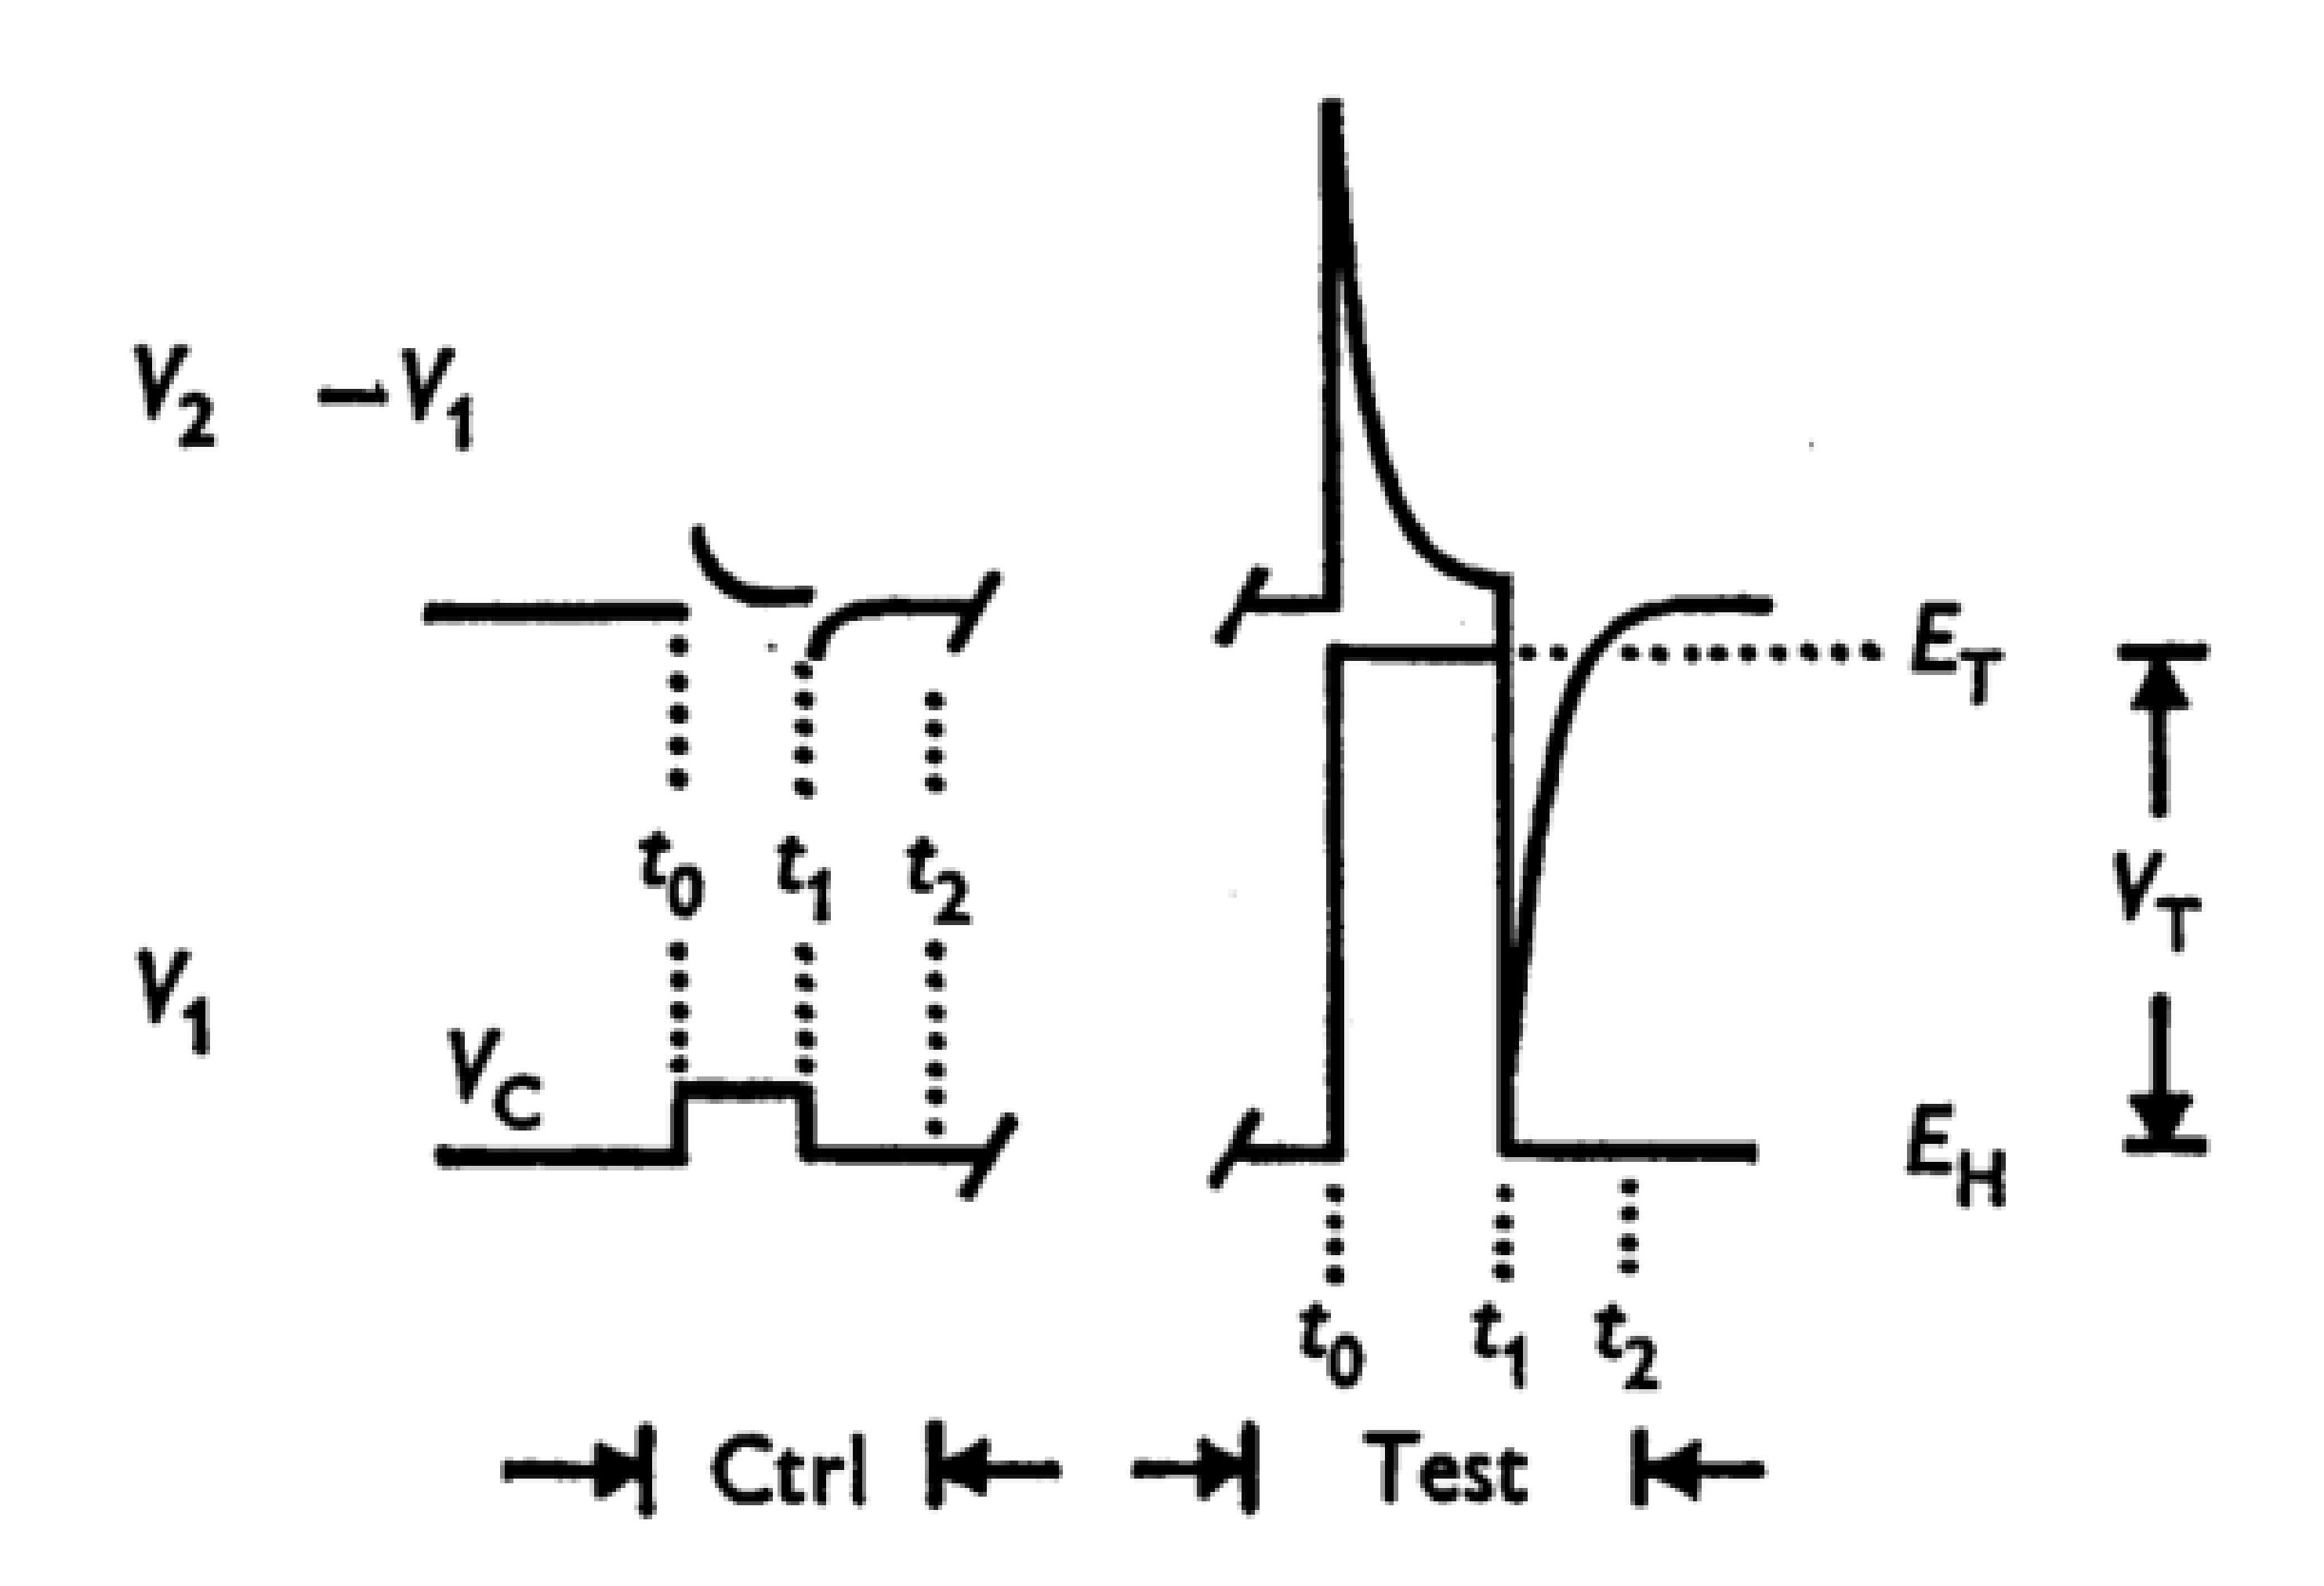
\includegraphics[height=6cm,
    angle=0]{./images/charge_movement_Adrian1976.eps}}
  \caption{$\Ca$ quarks}
\label{fig:charge_movement_Adrian1976}
\end{figure}

The depolarization of skeletal muscle fiber is accompanied a relatively small
non-linear component of membrane capacitive current that is attributed to the
movement of charged groups within the fibre membrane. So, intramembrane charge
movement was hypothesized as the voltage sensor. The on charge moved during the
depolarization is denoted as $Q_{on}$ and off charged moved during the
repolarization is denoted as $Q_{off}$ \citep{Melzer1986}.

\subsection{Molluscan neurons}

\citep{adams1979, kostyuk1981}

\subsection{Scorpion skeletal muscle}

\citep{scheuer1986}

\subsection{Heart}



In early studies, a slowly prepulse 500-ms from holding potential to prepulse
-50 mV, and keep -50mV for 50-ms, before applying the second test pulse is used
\citep{santana1996}. The reason of using a long prepulse to -50mV is that $\Na$
current is completely inactivated at this potential. After the test pulse, the
membrane was returned to -80mV. To isolate $\Ca$ current from other membrane
currents, a solution with 0Na 5 Ca external solution is used. To block ionic
currents, but allowing the measurement of charge movement, we use 0 Na, 4 Cd
solution. In a typical measurement, we see a rapid (positive) outward current
before (negative) inward $I_\ca$ current, before $I_\ca$ began to nominate the
recording $I_\ca$. $I_\ca$ reaches peak at the end of the 6-ms, and upon
repolarization, a tail current is observed. 

The test-pulse is used from -50mV to +10 mV \citep{hadley1991}, and they
splitted the outward transient current during depolarization into $Q_{on}$ and
inward transient during repolarization itno $Q_{off}$. The decline phase for the
tail current is about 0.65ms


To study $V_m$-dependent activation, a small duration of voltage step (6 ms or 7
ms) is used to produce maximal activation, yet to avoid rapid $\Ca$-dependent
inactivation. The reason is that the current reaches the peak by the end of 6-ms
step, and a tail current is seen upon repolarization. Then, another protocol,
with a 20-ms voltage-step is used to study charge movement. The analysis of
inactivation is complicated due to two inactivation mechanisms: $V_m$-dependent
and $\Ca$-dependent.

Voltage-clamp protocol with 7-ms step from -50mV holding with tespulse showed in
the figure from -40mV to +60mV in 0Na, 5Ca solution,
Fig.\ref{fig:LCC_Vm_activation_Hadley1991}. Here, the total cell capacitance was
assumed 50pF. NOTE: Large depolarization can cause vigorous contraction
(10\%-15\% cell shortening), but SR $\Ca$ was assumed normal due to the absence
of any spontaneous waves of CICR \citep{santana1996}.

\begin{figure}[hbt]
  \centerline{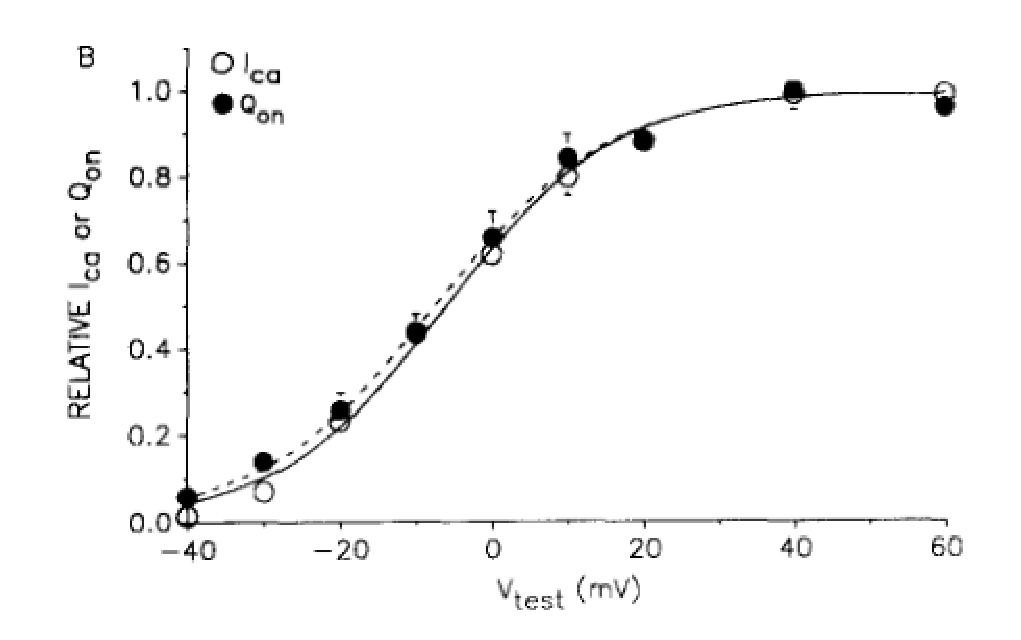
\includegraphics[height=7.2cm,
    angle=0]{./images/LCC_Vm_activation_Hadley1991}}
\caption{Normalized conductance-voltage relationship ($\Circle$) and
charge-voltage relationship ($\CIRCLE$). The solid curve is Boltzmann fit to
$I_\ca$ with $V_{1/2} = -6$ (mV) and $k = 11$ (mV). The dashed curve is
Boltzmann fit to $Q_\text{on}$ data with $V_{1/2} = -7.5$ (mV) and $k=11.5$ (mV)}
\label{fig:LCC_Vm_activation_Hadley1991}
\end{figure}

 

\section{Mechanism of activation/inactivation}
\label{sec:LCC_activation_inactivation}

In Purkinje fibre, using voltage-clamp (the clamp potential settled within 5ms,
then keep for the duration of 500ms)\citep{wier1982}, the current trace begins
with an outward spike (which changes direction after 8ms), then turn into a net
inward current. When the membrane is depolarized, $I_\CaL$ rises quickly to its
peak and gradually declines. The peak of the net inward current (reached after
15ms the start of depolarization) is about -100nA.  The underlying decay is called
``inactivation''. At the end of the voltage-clamp, the net current is outward
directed again, and then slowly declining this outward current after
depolarization, Fig.\ref{fig:LCC_current_Purkije_Wier82}.

Early review on this slow-inward current includes \citep{mcdonald1982} with a
bell-shaped curve of I-V relationship, showing a both activation and
inactivation phase. It's accepted that the channel is $V_m$-dependent
activation, i.e. the depolarization of the membrane potential ($V_m$) lead to
the transient inward $\Ca$ current ($I_\CaL$ rises quickly) and then decline
gradually. 
 
In early 1970s, the mechanism of inactivation was still in controversy with two
hypothesis: (1) Voltage-dependent \citep{bassingthwaighte1972cme}, (2)
[$\Ca$]$_i$-dependent \citep{linden1980,aronson1980}, or (3) both. 
The Hodgkin-Huxley-based formula of the current, based on the first
hypothesis, can be written as
\begin{equation}
I_\si = g_\si .d(V_m,t).f(V_m,t).(V_m-V_\si)
\end{equation}
with $d$ is activation variable, $f$ is inactivation variable. Using this
formula, the activation was first estimated to follow a mono-exponential time
course, with $\tau_d$ ranges from 5ms to 20-30ms for $V_m$ between -40mV to
+30mV in ventricular tissue \citep{reuter1973dcc} and shorter in SA-node
\citep{noma1980}. 

The idea that $\Ca$-sensitive inactivation was first discovered in Paramecium
\citep{brehm1978} which later was confirmed as a ubiquitous negative feedback
mechanism.  However, \textcolor{red}{with new experimental results, the
inactivation of DHPR is believed to be both $V_m$-dependent and
[$\Ca$]$_i$-dependent}, and
  first reported by \citep{lee1985icc}.
Nowadays, it's widely accepted that $I_\CaL$ is both $V_m$-dependent activation
and inactivation; and $\Ca$-dependent inactivation \citep{mcdonald1994}.
$\Ca$-dependent inactivation is the fast component, and $V_m$-dependent
inactivation is the slow component. 

\citep{hadley1991} suggested that the two mechanisms are independent. It implies
that the channel inactivated by voltage can also be inactivated further by $\Ca$
and vice versa. This can be modelled using two Inactivated states, each two for
$\Ca$ and $Voltage$. So, we need either 4 inactivated states, or three states in
which the first two inactivated states are both connected to the third
inactivated states. Check Sect.\ref{sec:LCC_Sun2000} for the latter case, and
Sect.\ref{sec:LCC_Mahajan2008} for the former case.

When using experimental data to estimate the prameters, it's suggested not to
use $\beta$-agonists as they have found to significantly effect on current
magnitude, voltage-dependent properties, and $\Ca$-dependent properties of the
channels \citep{faber2007DHPR}.

\subsection{CDI: Calcium-Calmodulin}
\label{sec:CaCM}

\textcolor{red}{\bf Experimental evidence}

the effect of
exogenous Ca2+ buffers and the type of buffer that can
interfere with CDI provide information about the distance
between the source of Ca2+ and the Ca2+-binding
site, and in turn, about the mechanism of CDI.

\textcolor{red}{\bf Biological mechanism}

Different hypotheses were proposed to explain how and where $\Ca$ affect LCC
\begin{itemize}
  \item How
  \begin{enumerate}
    \item {\bf shell model}: a 'shell' underneath the surface membrane of
    elevated $[\Ca]$ - a submembrane region \citep{standen1982bsm,chad1984},
    i.e. calcium current leads to a 'shell' of elevated $\Ca$ concentration
    underlying the entire plasma membrane; and the rate of filling this 
    shell govern the rate of $\Ca$ inactivation of the
    $\Ca$ current. Here, both open and closed channels in the shell
    experiences the same level of $[\Ca]$ so they have the same inactivation
    rate.
    
    \item {\bf pore model}: $\Ca$ channel pore experience a
    higher level of $[\Ca]$ \citep{sherman1990, Keizer1992}.
    Here, open channel has more $\Ca$, so the open channel are much more likely
    to be inactivated than closed channels.
    
    \item {\bf domain model}: a domain around the cytoplasmic entrance of the
    channel [ACCEPTED]: \citep{chad1986, yue1990csi, imredy1992scd, imredy1994mcs,
    deleon1995ecb}.
    
    \citep{deleon1995ecb} shown that there is consensus $\Ca$-binding motif,
    located on the $\alpha_{1C}$, called EF-hand motif can be a $\Ca$-binding
    inactivation site~\citep{deleon1995ecb} ($\Ca$-induced exposure of
    hydrophobic residues on the E and F helices, which could then interact with
    a complement hydrophobic surface to inhibit opening). EF-hand region of
    L-type $\Ca$ channel (LCC), not in the conduction pore, can be a potential
    locus for inherited electrical disorders like long QT syndrome. In addition,
    EF-hand can  be a new molecular target for inotropic and anti-arrhythmic
    drugs. \citep{qin1999} narrowed down this region into a shorter segment 
    located downstream of the EF-hand, containing 144 a.a. and called RL-VS
    (denoting the begining and the ending amino acids). In the middle of the
    RL-VS sequence is an 8 a.a. sequence with an {\bf IQ motif}.
    
  \end{enumerate}
  \item Where
  \begin{enumerate}
    \item direct $\Ca$ binding to the channel: \citep{sherman1990,
    Keizer1992,standen1982bsm}
    \item $\Ca$ induce channel (de)phosphorylation: \citep{chad1986,
    armstrong1989}
    \item $\Ca$ activation of calmodulin [ACCEPTED]: \citep{chad1986,
    armstrong1989, peterson1999}. Calcium-free CaM is called Apocalmodulin
    (Sect.\ref{sec:calmodulin}), while calcium-bound calmodulin is denoted as
    Ca/CaM complex \citep{jurado1999}. However, where Ca/CaM acts ??? (return to the
    information given above, i.e. the EF-hand motif) The detailed mechanism is
    given below
  \end{enumerate} 
\end{itemize} 

Nowadays, the underlying cellular mechanism of calcium-dependent inactivation is
through the binding of calcium to calmodulin, the direct sensor of inactivation.
Calmodulin (CaM or CM), i.e. CALcium-MODULated proteIN, belongs to the Troponin
C superfamily of high-affinity calcium-binding proteins. Each CaM molecule has 4
calcium-binding sites (the EF-hand: 4 homologous domains, each with one
$\alpha$-helix-calcium binding loop) \citep{kretsinger1980}. NOTE: The EF-hand
here is different from the EF-hand motif in $\alpha_\text{1C}$ in LCC.
 
Given that Calmodulin regulates L-type calcium channel. It is clearly that
without the IQ motif, the CDI is removed \citep{qin1999}. However, the question
is the mechanism.Three hypothesises were given \citep{ehlers1999calm}.
\begin{enumerate}
  \item CaM bind to IQ motif all the time, when $[\Ca]$ elevates, $\Ca$ binds to
  CaM to trigger the inactivation.
  
  \item CaM bind to IQ motif all the time, when $[\Ca]$ elevates, $\Ca$ binds to
  CaM that cause $\Ca$/CaM to move to the {\it effector site} - where it really
  trigger the inactivation.
  
  \item CaM bind to the some other {\it tethering site} (not the IQ motif), when
  $[\Ca]$ elevates, $\Ca$ binds to CaM that cause the conformational change that
  allow $\Ca$-CaCM to bind with IQ motif to trigger the inactivation.
\end{enumerate}

It was found that Calmodulin tether to the channel, but not affect the channel;
until $\Ca$ bind to calmodulin, forming CaCaM complex, then CaCaM inhibit the
opening of the channels. So, depending on the assumed model, IQ-motif can
function as a tether (option 2), an effector site (option 3) or both (option 1).
Knowing these will help to understand the effect of mutation in
structure-function relations of $\Ca$-sensitive inactivation.
CaM is the actual $\Ca$ sensor for inactivation \citep{peterson1999}. The CaM
tethers with L-type $\Ca$ channels at the C-terminus, independent of
$\Ca$-binding to CaM. The reason is that the half-maximal binding of CaM to the
RL-VS region is 0.37$\muM$ of calcium concentration, which is enough at resting
level \citep{qin1999}. In the absence of $\Ca$, the C-terminus-CaM complex is
hypothesized to act as a brake on the ability of inactivation gate (to
inactivate the channel) which locate at the cytoplasmic I-II linker
\citep{mahajan2008}.

\begin{framed}
The inactivation dependence of $\Ca$ channel to divalent cations were
tested with $\Ca$, \ce{Sr^2+} and \ce{Ba^2+}, correspondingly as
external ions. \textcolor{red}{The inactivation was most sensitive to $\Ca$, to
a lesser extent to \ce{Sr^2+}, and the least to \ce{Ba^2+}} by looking
at the change in the time-course of the inactivation.
\end{framed}


\begin{framed}
At first, it was assumed that the inactivation is dependent upon bulk myoplasm
calcium. Later, based on local control theory~\citep{wier1994lce}, DHPRs
inactivation depends on a local change of concentration of calcium $[\Ca]_\ds$,
rather than the cytosolic one $[\ca]_i$
\citep{bers1991ecc,cheng1993cse}.  The rate of inactivation can be
controlled, for a given voltage clamp, by grading the amount of $\Ca$
entry \citep{wier1999}. 

\end{framed}

When $\Ca$ binds to this tethered CaM, $\Ca$ induces conformational change, i.e.
the $\Ca$/CaM complex interacts with the IQ-like motif at the carboxyl end
tail of $\alpha_{1C}$, Fig.\ref{fig:LCC_diagram}. This binding removes CaM from the
brake site, allowing I-II linkers to inactivate the channel more rapidly. The
region for $\Ca$-dependent inactivation is called putative EF hand or an IQ-like
motif for CaM binding. CaM contains 4 calcium-binding domains with an
E-helix-loop-F-helix repeat. It's suggested that 3 to 4 calcium ions is required
for the activation of CaM \citep{cox1988}. \textcolor{red}{The LCC remains in
this non-conducting state until the inactivation process is reversed in the
event of a decrease in $[\Ca]_i$.} So, in modelling, the backward rate constant
from calcium-inactivated state to opening state is set to a small value.

\begin{figure}[hbt]
  \centerline{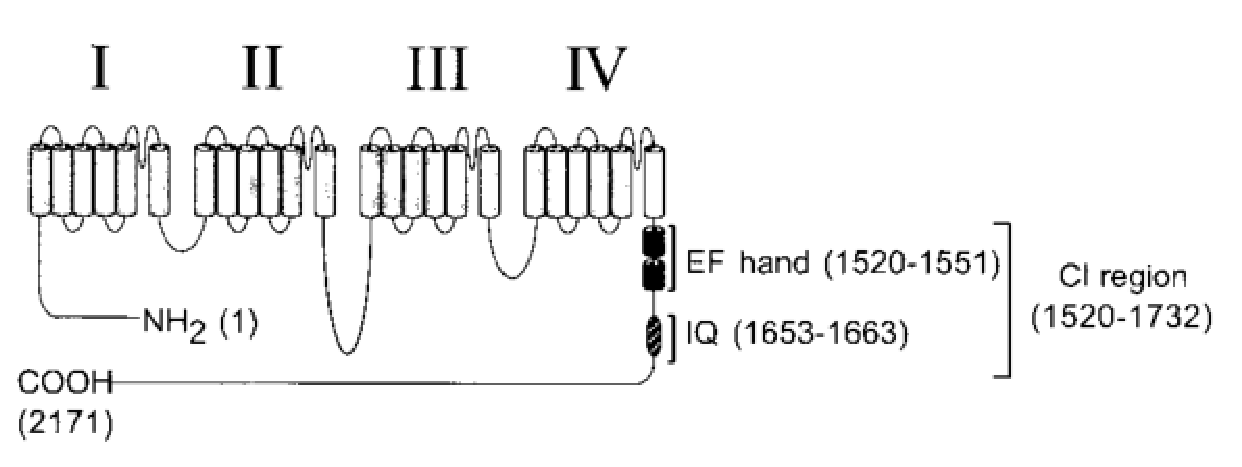
\includegraphics[height=4cm,
    angle=0]{./images/LCC_diagram.eps} }
  \centerline{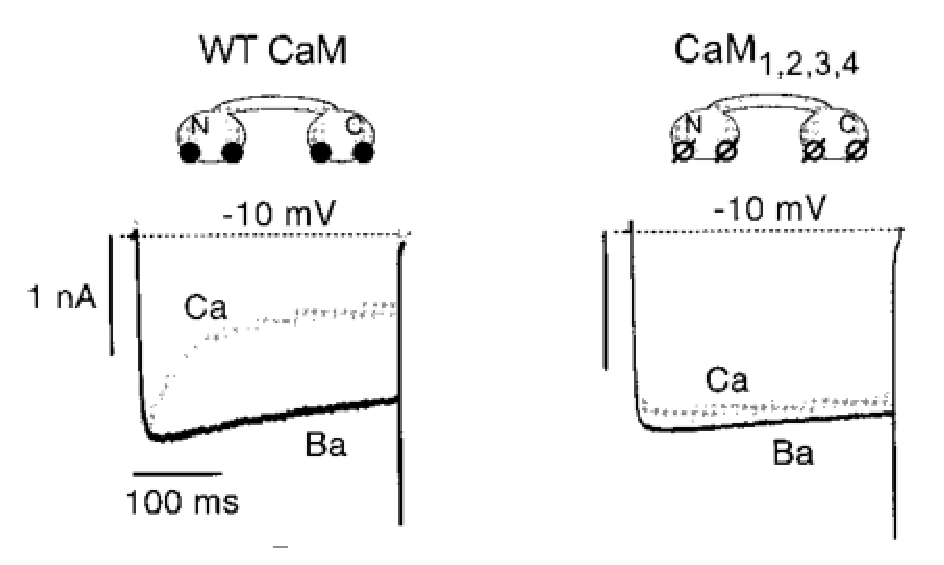
\includegraphics[height=4cm,
    angle=0]{./images/LCC_Ca-dependent_inactivation.eps} }
\caption{ (A) CI region of the cytoplasmic -COOH tail has a region important for
$\Ca$-dependent inactivation; (B) Evidence of $\Ca$-dependent inactivation
(using depolarization step -10mV)}
\label{fig:LCC_diagram}
\end{figure}

As shown in Fig.\ref{fig:LCC_diagram}(B), when $\Ba$ is used as the charge
carrier, it doesn't have the significant reduction in currents. Here, the effect
of $\Ba$-dependent inactivation exist, but very small. Also, when CaM is
knockout (i.e. suppressing high-affinity $\Ca$ binding sites), the effect of
$\Ca$-dependent inactivation is removed as well. \textcolor{red}{At 180ms after
the voltage-clamp, the inactivation should be completed} \citep{rose1992}. 

\begin{framed}
Interestingly, CaM can also bind to analogous IQ regions on other memmbers of
the channel family (N-, P/Q-, and R-type of $\Ca$ channels) in a $\Ca$-dependent
manner as well. However, the lack of $\Ca$-dependent inactivation suggests that
it's the result of a failure to transduce CaM binding into inactivation, rather
than the failure to bind CaM.

\end{framed}

The rate of $\Ca$ binding to CaM is very fast. It was suggested that CaM has
four calcium binding sites. There are two hypothesis \citep{cox1988}
\begin{enumerate}
  \item The four binding sites have very similar affinities
  \item Two pair of sites with pronounced positive co-operativity within each
  pair and a marked difference in affinity between the pairs. One pair (at
  N-terminal) with high $\Ca$ affinities  and the other pair (at C-terminal)
  with low $\Ca$ affinities \citep{martin1985}. 
\end{enumerate}
Many studies favour the latter model. If we assume the fast binding sites are
always occupied, and only consider the low-affinity sites, with $K_d \approx
10\muM$ \citep{jurado1999}.

The reaction of $\Ca$ with Quin-2 is very much faster than the dissociation of
$\Ca$ from CaCM so it can be used as a kinetic indicator. \citep{martin1985}
used Quin-2 buffer to induce the dissociation of $\Ca$ from $\Ca_4$-CaM complex
(CaCM) in the presence of 0.1M KCl, and in the tempperature range
11.3-30.1$^\circ$C. The effect of 0.1M KCl is to accelerate the slow process by
a factor of $\approx 2$, while the fast process is slowed by $\approx 3$.
\begin{enumerate}
  \item low affinity sites C-terminal ($k_\off$=10-40 s$^{-1}$): $k^\off =
  9.1\pm 1.5$ (1/s) (without KCl), $k^\off = 24\pm 6.0$ (1/s) (with KCl)
  \item high affinity sites N-terminal ($k_\off$=300-500 s$^{-1}$): $k^\off =
  650$ (1/s) (without KCl), $k^\off = 240\pm 50$ (1/s) (with KCl) 
\end{enumerate} 
So, $k_C=10k_N$ ($k_C$=at C-terminal, $k_N$=at N-terminal).

It was assumed that a diffusion controlled on-rate constant of $k^\on=10^2$
($\muM^{-1}$.s$^{-1}$) the same at both types of binding sites
\citep{eigen1962}. It's suggested that the high-affinity complex ($K_d=1$nM) is
only formed if at least three calcium ions bind to CaM. So, the $K_d$ difference
is about 10-20x. However, if the $\Ca$-on-rates are different as well, then
there's no difference  in $K_d$ between the two types of  $\Ca$-binding sites. 


\begin{figure}[hbt]
  \centerline{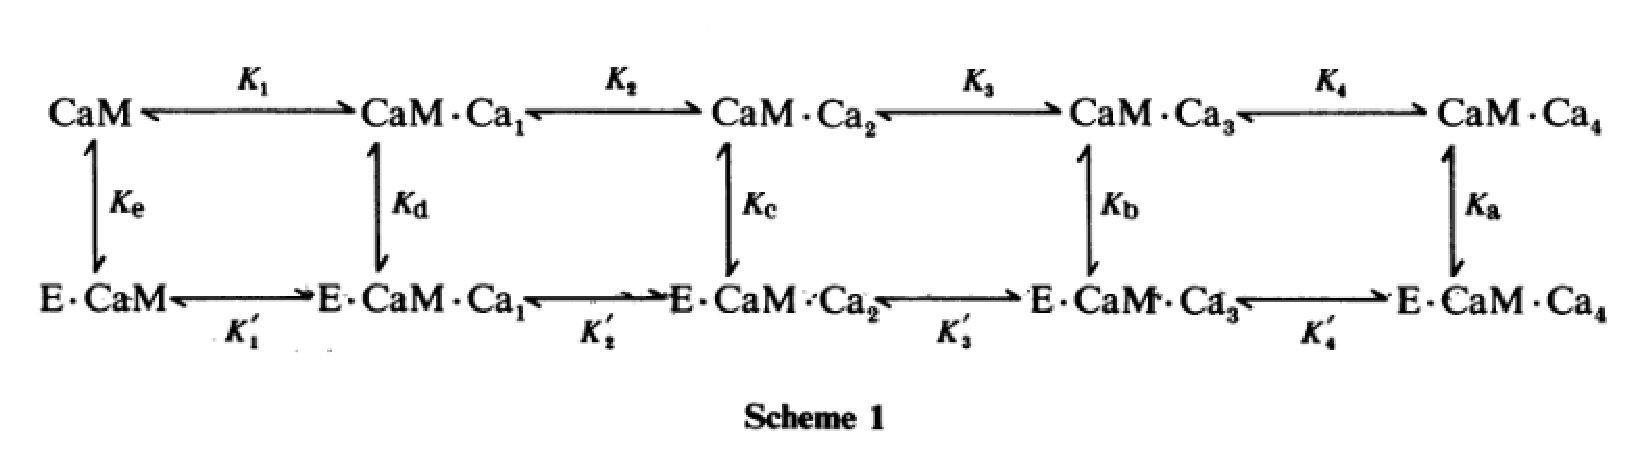
\includegraphics[height=4cm,
    angle=0]{./images/Enzyme_CaCM_scheme.eps} }
\caption{A scheme of energy coupling in the interaction between CaM, $\Ca$ and
the enzyme \citep{cox1988}. Here, there are 9 independent parameters: }
\label{fig:LCC_diagram}
\end{figure}

So, at the early rising of $[\Ca]$, calcium first binds to the C-terminal half
of CaM, and later to two lower-affinity binding site (domains I and II)
\cite{cox1988}. The energy barrier for
\begin{enumerate}
  \item dissociation of one $\Ca$ ion: $\Delta G_d=$ 59 kJ/site
(fast) and 67  kJ/site (slow).
\item association of one $\Ca$ ion: $\Delta G_a=$ 30 kJ/site (fast) and 38
kJ/site (slow).
\end{enumerate}


CDI in L-type calcium channel has widely known to be PKA dependent. However,
there are evidence that it can also be G protein-coupled receptors dependent in
which G-beta-gamma (G$\beta\gamma$) is believed to affect CDI of L-type
calcium channel \citep{ivanina2000}. G$\beta\gamma$ has direct interaction with
C-terminal of L-type $\Ca$ channel \citep{qin1997}.

Calmodulin not only mediate $\Ca$-dependent inactivation, but also {\it
facilitation} (Sect.\ref{sec:facilitation_CaMKII}). 
  
\subsection{VDI}

VDI is affected by mutatios to the pore-encoding portions of the channel
\citep{stotz2001} or the mutations within the I-II linker \citep{splawski2004,
dafi2004}.  The VDI is completely eliminated in Timothy syndrome, with G406R
missensed mutation.

There has been recent evidences that VDI may also dependent on the IQ-CaM
complex \citep{liang2003}, giving rise to the possibility that VDI and CDI are
not entirely independent. That's why some models assume the two inactivated states
(in each mode), or the two modes connecting to the same third inactivated
states. 

It's suggested that the channel has two kinetics: fast and slow
voltage-dependent \citep{ferreira2003}. 

\subsection{Time course of activation/inactivation}
\label{sec:LCC_timecourse}


The activation and inactivation time constant was fitted using Boltzmann
function. The theoretical curve was fit to the data using Marquardt algorithm,
to determine $V_{1/2}$ and $k$ of the Boltzmann function for best fitting
exponential curve. See next section for the experimental procotol
(Sect.\ref{sec:double_pulse_protocol}).

Inactivation of $I_\CaL$ is biexponential when $\Ca$ is the charge carrier and
mono-exponential when $\Ba$ is the charge carrier. So, many models model the
inactivation in two pathways: VDI and CDI (Calcium-dependent Inactivation and
Voltage-dependent inactivation). 



\subsection{Double-pulse protocol}
\label{sec:double_pulse_protocol}


\begin{framed}

The double-pulse protocol is typically used to study steady-state inactivation
\citep{hadley1987}. From the resting potential (holding potential), a prepulse
is applied (tested with different value of conditioning potentials, and at the same duration). The prepulse
duration was chosen for particular experiments to induce calcium-sensitive
inactivation. Then, the next pulse is used to test the readiness of L-type $\Ca$
channels after inactivated.

After the prepulse, the channel is brought back to holding potential for 10-ms
before applying a test pulse. For each trial, a different concentration of
agonist (say Bay K 8644(-)) is used, e.g. 40, 100, 500nM, and 2$\muM$. In
Purkinje fiber, the holding potential is -50mV. In rat ventricular myocyte, the
holding potential is -80 mV, then various prepulse potential for 400 ms, then to
step pulse 0 mV for 100ms and finally clamped back to the holding potential
\citep{sun2000mlc}. Here, the interval separating the prepulse and step-pulse
was eliminated to avoid time-dependent recovery from inactivation and also to
maximize voltage-dependent effect. It also avoid $\Ca$ tail currents during the
interval that could lead to additional inactivation.

\end{framed}

\citep{imredy1994mcs} used patch-clamp to measure single channel. Prepulse
protocol: hold the patch at -50 mV, after which a prepulse +20 mV is applied for
100ms. A ``control" protocol: bring the patch back at -80 mV for 20 ms before
applying the testpulse +20mV for 400ms. Each prepulse protocol is alternated
with a control protocol. This will give us the data of current in both absence
and presence of $\Ca$ prior $\Ca$ entry, Fig.\ref{fig:Imredy_Vclamp}. The
interpulse -80 mV can drive the channel to the left-most close state.

\begin{figure}[hbt]
  \centerline{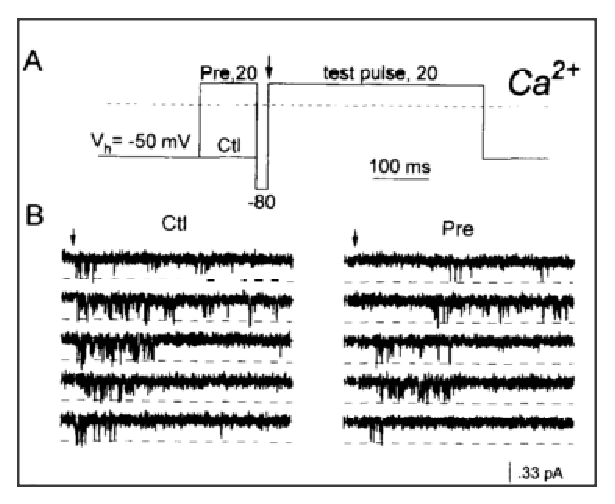
\includegraphics[height=5cm,
    angle=0]{./images/Imredy_Vclamp.eps}}
  \caption{(A) V-clamp method; (B) Channel recording}
\label{fig:Imredy_Vclamp}
\end{figure}

The threshold for triggering the channel lies positive to -50mV in ventricualr
tissue, while in SA-node, it maybe negative to -60mV \citep{noma1980}.
Stepping the voltage from holding potential -50 mV to +20 mV, the time course
$\tau$ of $P_o$ was obtained from averaging several records by fitting a
monoexponential function \citep{yue1990csi}. The dependence of $\tau_f$ on
voltage was first assumed to be with an exponential time course, then was
revised to be a bell-shaped with the maximum near -15mV (or more precisely to be
a U-shaped with a minimum near -25mV) \citep{mcdonald1982}.

\section{CDF (calcium-dependent facilitation): CaMKII }
\label{sec:facilitation_CaMKII}

There are many $\Ca$-dependent proteins that contribute to the fine tuning of
ECC. One of them is CaMK, with the predominant cardiac isoform is CaMKII
(Sect.\ref{sec:CaMKII}).
We know that $\Ca$-dependent inactivation occurs via $\Ca$-bound calmodulin
(Ca2+/CaM). However, at high frequency of pacing rate, the LCC also exhibits
$\Ca$-induced potentiation or facilitation. This cannot be detected using
voltage-clamp or prepulse \citep{brette2006cc}. 

At high frequency, peak $I_\CaL$ is slightly increase, and (higher impact) the
process of inactivation is slower \citep{carmeliet2004}. Biologically, this
facilitation process is the result of activation of CaMKII that
phosphorylate the C-terminal of the $\alpha 1$-subunit
\citep{yuan1994, wu2001} or $\beta$-subunit \citep{Grueter2006}.
Facilitation and inactivation may occurs simultaneously \citep{hirano1994}.
\textcolor{red}{The physological role of facilitation is still not clear; yet
it may offset to some degree the $\Vm$-inactivation at higher pacing rates}.

Incorporating CaMKII to the model of LCC and other proteins is considered
important, as altering CaMKII signaling pathway is thought to shape the
phenotype of heart failure (HF) \citep{}, e.g. 
\begin{itemize}
  \item acute overexpression of CaMKII (in isolated rabbit ventricular
  myocytes): increase $\Ca$ spark frequency and enhanced frequency-dependent acceleration
  of relaxation. Its expression is increased in human heart failure in both
  ischemic and dilated cardiomyopathy \citep{hoch1999, kirchhefer1999}. It's
  believed caused by the impaired ejection fraction, i.e. instead of pumping
  out via NCX, there's an increase in SR uptake via SERCA pump (mainly through
  PLB phosphorylation). However, transgenic overexpression of $\delta_C$ isoform
  (CaMKII$\delta_C$) lead to reduced SR $\Ca$ content and thus causing altered
  intracellular $\Ca$ handling.

  \item elevated CaMKII activity (in transgenic mice): increase AP duration,
  decrease twitch shortening, and leading to dilated cardiomyopathy \citep{}.
\end{itemize} 

When $[\Ca]_i$ increases during systole, $\Ca$ bind to CaM (upto 4 calcium ions
per CaM), then Ca2+/CaM complex binds to the regulatory domain of CaMKII and
displaces the autoinhibitory domain on CaMKII, thereby activating the enzyme.
EC50 for the activation (i.e. half maximal activation) is at
$[\Ca]_i=0.5-1\muM$. After activated, CaMKII can lock itself in the activated
state upon autophosphorylation which allow CaMKII to maitain the active state
even after $[\Ca]_i$ has declined. Even though autophosphorylation is not
essential for the activating of CaMKII, it does increase the affinity to CaM
($\approx 700x$, i.e. $K_d$  decreases from 45nM to 60pM) \citep{braun2005},
trapping CaM \citep{meyer2006}. Remember that the resting level
$[\Ca]_i=100$nM, so CaM is still trapped for several seconds.

%\chapter{\texorpdfstring{$\Ca$ channel models}{Ca2+ Channel Models}}
\section{Hodgkin-Huxley-based LCC model}

This section focus on LCC model that use Hodgkin-Huxley-based formula.

It is assumed that the $\Ca$ current follows a linear relationship with the
membrane potential, i.e. the whole-cell ionic current can be calculated as the
fraction of opening channels times the maximum conductance times ($V_m-E_i$). 
The fraction of opening channels can be represented as the result of the product
of some gating variables.
\begin{itemize}
  \item $d$ = voltage-dependent activation
  \item $f$ = voltage-dependent inactivation
  \item $f_2$ = calcium-dependent inactivation
\end{itemize}

In Hodgkin-Huxley scheme, the gating variables are independent of each other.
However, it was showed that the strong coupling between kinetic transitions
cannot be reproduced with Hodgkin-Huxley paradigm \citep{rudy2006}.

Also, Hodgkin-Huxley formalism does not represent kinetic states of the
individual ion channels (open, closed, inactivated) and is therefore not
suitable for simulating molecular interactions, ion-channel mutations that alter
specific kinetic transitions, or effect of drugs that bind to the channel at a
specific conformational state. The solution is to use Markov-models which will
be described in the next sections.

\subsection{Beeler-Reuter (1977)}

There were evidences that LCC pemeate not only calcium, but also other ions.
Even though, for simplicity, \citep{beeler1977rap} assumed LCC is selective only
to $\Ca$. The channel is assumed to be activated and inactivated by membrane
potential
\begin{equation}
I_\si = \bar{g_\si}.d.f.(V_m-E_s)
\end{equation}
with two gating variables $d(V_m,t)$ (activation) and $f(V_m,t)$ (inactivation)
(Sect.\ref{sec:beeler-reuter-model}).

\subsection{Ashcroft-Stanfield (1982)}

Ashcroft-Stanfield assumed that LCC increase with $[\Ca]_o$, and is inhibited by
$[\Ni]_o$ \citep{ashcroft1982cis, ashcroft1982}. Also, the current reach the
maximum value at a certain value of $[\Ca]_o$. To formulate that the Ca-current
is saturated when $[\Ca]_o$ is high enough that most likely all binding sites
are bound, ~\citep{ashcroft1982} used the simple formula
\begin{equation}
  \label{eq:1074}
  I_\ca(V_m) = \frac{I_{\max,\ca}(V_m)}{1+\frac{K_\ca(V_m)}{[\Ca]_o}}
\end{equation}
with $K_\ca(V)$ is the dissociation constant for the binding site. At
$V_m=0$mV, $K_{\max,\ca}(0)=7.3$mM,
$I_{\max,\ca}(0)=-226\mu$A.cm$^{-2}$. 


It was hypothesized that there is a number of binding sites on the extracellular
side of the channels. To model the effect of Ca-channel inhibitors, say
$\ce{[Ni]_o}$, that potentially completely block Ca-current when $[\ce{Ni}]_o$
is high enough to occupy the binding sites,~\citep{ashcroft1982} used the
formula
\begin{equation}
  \label{eq:1075}
  I_\ca(V_m) =
  \frac{I_{\max,\ca}(V_m)}{1+\frac{K_\ca(V_m)}{[\Ca]_o}\times \left(1+\frac{[\ce{Ni}]_o}{K_\ni(V)} \right)}
\end{equation}
As Ni bind twice as strong as Ca, we have $K_\ni$ is about half of
$K_\ca$, e.g. $K_\ni=3.7$mM at $V_m=0$mV. 

\subsection{Standen-Stanfield (1982)}

Experimental data shown that $V_m$-dependency show a biphasic behavior (i.e.
both activation and inactivation). However, modelling $V_m$-dependent activation
and inactivation {\it per se} cannot fit the experimental data. It was then
suggested that $\Ca$-dependent inactivation should be considered. For the first
time, a formula for LCC with $\Ca$-dependent inactivation was given by
\citep{standen1982bsm} (Sect.\ref{sec:standen_1982model}). However, the model
ignore voltage-dependent inactivation. \textcolor{red}{[CONS: no
Voltage-dependent inactivation]}
 
Also, it's widely accepted that LCC permeate multiple ions; so GHK-equation
(constant-field theory) is being used as well.
\begin{equation}
I_\CaL = \bar{P_\ca}.m^3.h.\frac{z_\ca ^2V_mF^2}{RT} \left[
     \frac{ \gamma_{o}[\ca]_o-\gamma_{i}[\ca]_i\exp(z_\ca V_mF/RT)}{1-\exp(z_\ca V_mF/RT)}\right]
\end{equation}
with $m(V_m,t)$ (activation) and $h([\Ca]_i,t)$ (inactivation).


\subsection{DiFrancesco-Noble (1985 - Purkinje fibre)}
\label{sec:difr-noble-1985}

Later on, it was found that LCC is not selective to $\Ca$ only. There are other
ions that can permeate through LCC as well. \citep{difrancesco1985mcea}
explicitly describe the current through LCC (on Purkinje fibres), $I_\si$ as the
sum of three separate ionic currents: Ca, K, and Na. [NOTE: In their previous
model, only the first two ions $\Ca, \Na$ were considered
\citep{reuter1977sic}.]
\begin{equation}
  \label{eq:864}
  I_{si} = I_{\ce{Ca}} + I_{\ce{Na}} + I_{\ce{K}} \;\;\;\text{(nA)}
\end{equation}
Then, the reversal potential of LCC is estimated using GHK-based equation
\begin{equation}
  \label{eq:862}
  E_{Ca} = \frac{RT}{F} \ln \left( \frac{
      4P_{\ce{K^+}}\ce{[K^+]}_{out} +  P_{\ce{Na^+}}\ce{[Na^+]}_{out} +  P_{\ce{Ca}}\ce{[Ca]}_{out} 
    }{ 4P_{\ce{K^+}}\ce{[K^+]}_{in} +  P_{\ce{Na^+}}\ce{[Na^+]}_{in} +  P_{\ce{Ca}}\ce{[Ca]}_{in} 
    } \right)
\end{equation}
with the permeability of $\Ca$ ions $P'_{\ce{Ca}}$.
\begin{equation}
  \label{eq:863}
  P'_{\ce{Ca}} = P_{\ce{Ca}} \left[ \frac{1}{\exp(\frac{V_m - V'}{RT/F}) +
      1 }\right] 
\end{equation}
$V'$ is the fixed charge potential (resulting from the relative distribution
of fixed surface charges in the vicinity of the respective ion
channels on both sides of the membrane). The relative permeability for the three
ions are represented via the ratios $P_{\ce{Ca}}/P_{\ce{Na}} = 1/0.01$,
$P_{\ce{Ca}}/P_{\ce{K}}=1/0.01$. 

The three gating variables were: $d$ voltage-gating
activation variable, $f$ voltage-gating inactivation variable, $f_2$
$\Ca$-dependent inactivation variable \citep{difrancesco1985mcea}
(Sect.~\ref{sec:difr-noble-purk}).

\subsection{Rasmusson et al. (1990)}
\label{sec:LCC_Rasmusson1990}

\citep{rasmusson1990mme, rasmusson1990mms} modelled L-type $\Ca$ current using
two gating variables, without calcium-dependent inactivation
\begin{equation}
I_\ca = d.f.\bar{I}_\ca
\end{equation}
with
\begin{equation}
\bar{I}_\ca = \frac{0.01174 V_m \left( [\Ca]_i \exp(0.07792 V_m) -
[\Ca]_o \right)}{\exp(0.07792 V_m) - 1}
\end{equation}

The two gating variables have the time constant and equilibrium values as given
below
\begin{eqnarray}
1/\tau_d &&= \frac{0.035 (V_m + 10)}{d_\infty \left( 1- \exp (- (V_m + 10)
/ 6.24\right)} \\
d_\infty &&= 1/ \left(1+ \exp(- (V_m + 10) / 6.24 \right) \\
1/\tau_f &&=  0.0197 \exp(-(0.0337(V_m+10))^2)) + 0.02 \\
f_\infty &&= \frac{1}{1+ \exp((V_m + 35.06)/8.6} + r 
\end{eqnarray}
with 
\begin{equation}
r = \frac{0.6}{1 + \exp((50-V_m)/20)}
\end{equation}

The model was developed using SV cell data from \citep{Hume1981}. The peak was
reduced to account for the lower peak (2.0-2.5x smaller) in bullfrog atrial cell
vs. SV cell, i.e. at $[\Ca]_o=$2.5mM, peak $I_\ca$ = 200pA  at 0mV in atrial vs.
500pA in SV cell. 

The time constant of the inactivation term $\tau_f$ doesn't have the
conventional bell-shaped function of $V_m$, but a nonmonotonic U-shaped
dependence upon $V_m$. The steady-state inactivation $f_\infty$ has also a
monotonic U-shape dependence on $V_m$, i.e. $f_\infty$ decrease when $V_m$
depolarized until +20mV and then it becomes reactivating (increase) if $V_m$
continues to increase (> +20mV).




\subsection{Luo-Rudy (1994)}
\label{sec:LCC_Luo1994}

\citep{luo1994dmc_a} incorporates the inactivation by both $\Ca$ and voltage.
Also, to account for multi-ion permeability across L-type $\Ca$ channels, they
used GHK equation with a large permeability for $\Ca$ and a smaller permeability to
$\Na$, $\K$. Using GHK equation, the permeations through the channels of
different ion species are assumed to be independent
(Sect.\ref{sec:luo-rudy-phase-2}).

\section{Hess et al. (1984,1986) - mode switching}
\label{sec:LCC_Hess1984}

Hess et al. didn't proposed a particualr working mode, but a mechanism of gating
known as {\bf mode switching}. To help record more accurate measurement of small
unitary currents, Bay K 8644 was used to obtain long-lasting openings of LCC,
Fig.\ref{fig:BayK8644}. The contribution from T-type $\Ca$ channels was
assumed insignificant and was ignored.

\begin{figure}[hbt]
 \centerline{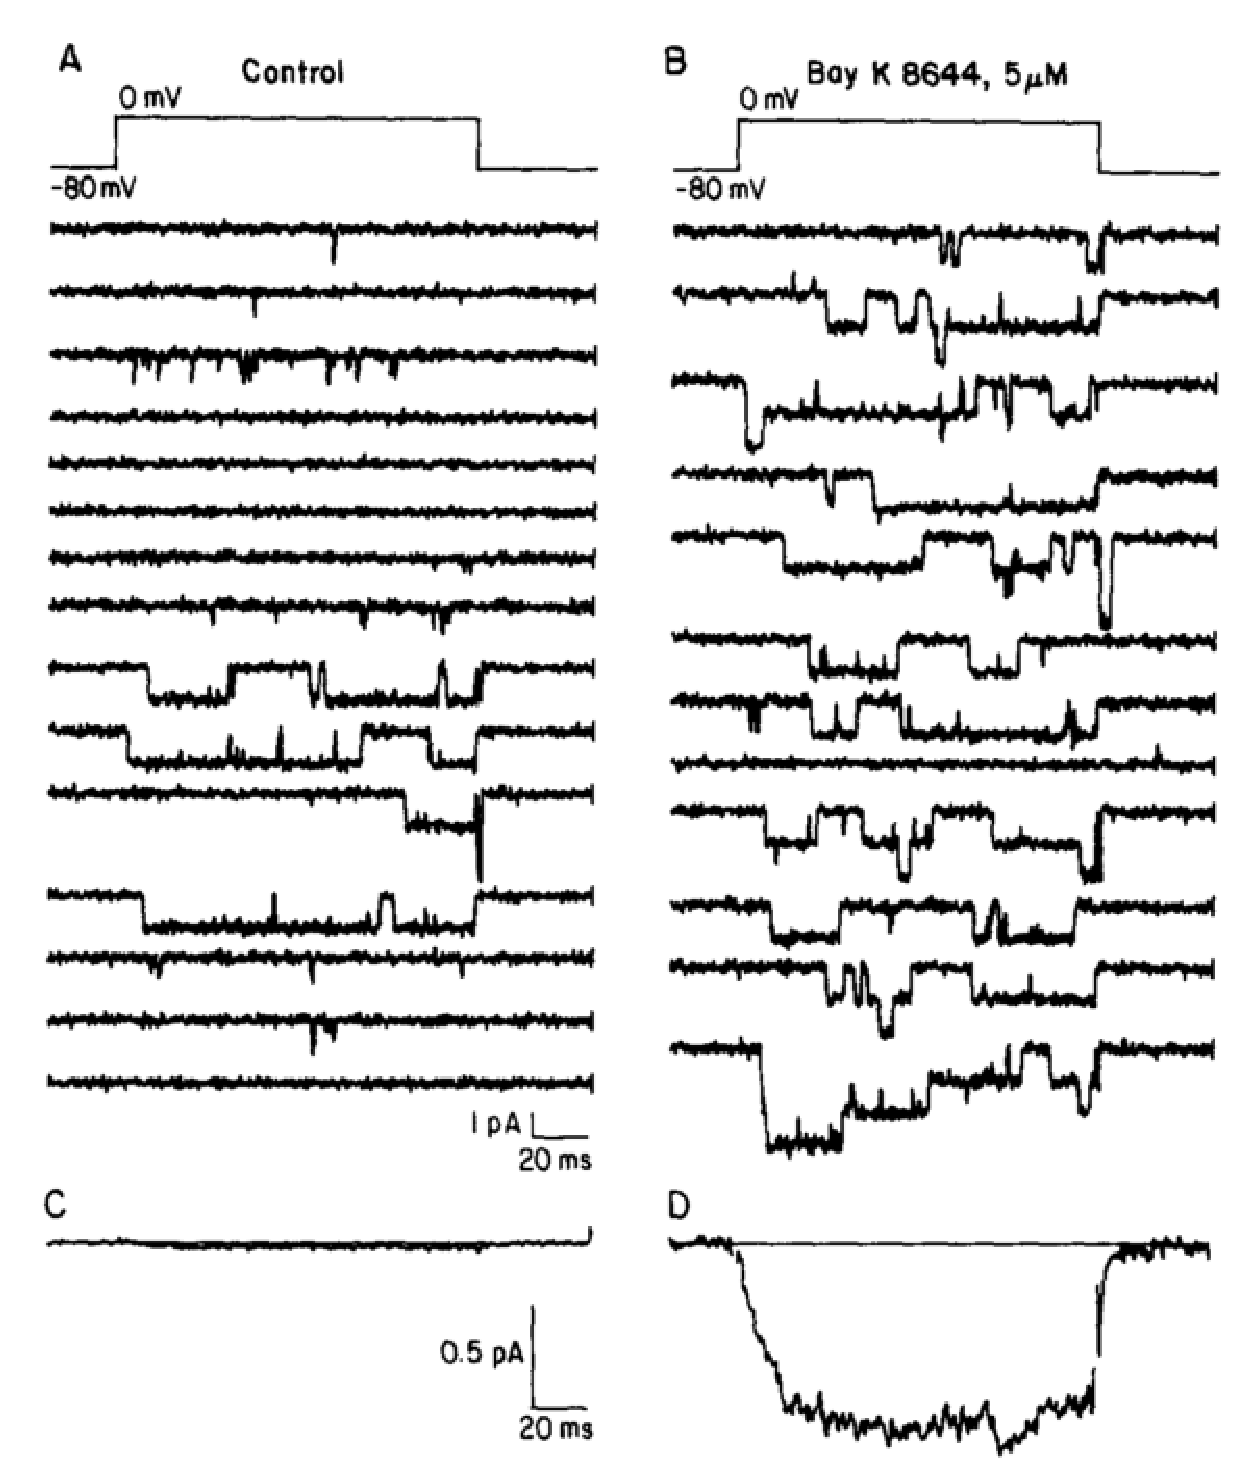
\includegraphics[height=7cm, angle=0]{./images/BayK8644.eps}}
\caption{Bay K 8644 increase the proportion of channel switching with
  long-lasting openings.}
\label{fig:BayK8644}
\end{figure}

The $\Ca$-sensitive in gating requires a different approach rather than
Hodgkin-Huxley formalism. Even though they didn't introduce a particular working
model, \citep{hess1986ccs} suggested a three mode model,
Fig.~\ref{fig:Hess_mode}

\begin{figure}[hbt]
 \centerline{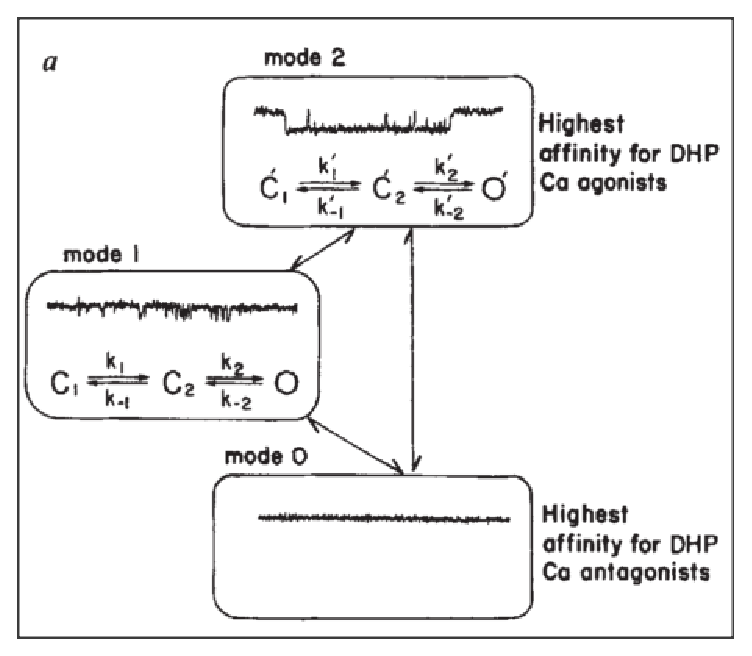
\includegraphics[height=7cm, angle=0]{./images/Hess_mode.eps}}
\caption{3 modes of $\Ca$ channels}
\label{fig:Hess_mode}
\end{figure}

\begin{itemize}
\item mode 1: a brief opening ($\sim$ 1ms) and burst (switching between short
closed and opening)
\item mode 2: much longer opening interrupted by brief closure
  appeared very rarely
\item mode 0: no opening at all
\end{itemize}
Mode 0 is favoured by $\Ca$ antagonist nitrendipine and
nimodipine. Mode 2 is favoured by $\Ca$ agonist Bay K 8644 (which bind to $\Ca$
and thus reduces the number of free $\Ca$ that can bind to L-type
$\Ca$ channels to inhibit the opening). Mode 1 and 2 both have two closed state
and one open state; each with different rate transition.
\begin{equation}
  \label{eq:989}
  I \ce{<=>} C \ce{<=>} O
\end{equation}

\citep{hess1986ccs} summarized:
\begin{enumerate}
\item Suggest multiple modes of $\ca$ channels: Due to the complex structure of
the channel, \citep{hess1984} suggested using multiple
state model formalism to better represent the kinetics of the channels. One way
is the {\bf ``modal switching'' approach} in which the kinetics of the  channels
is characterized by different modes. 

\item New ranking of ion permeability: $P_{\ce{Ca}}/P_{\ce{Cs}} > 1000$,
$P_{\ce{Ca}}/P_{\ce{K}}>1000$. The  relative selectivity for divalent ions are: $\Ca
> \ce{Sr^2+} >  \ce{Ba^2+} \gg \ce{Mg^2+}$.  The relative selectivity for
monovalent  ions are: $\ce{Li+} > \ce{Na+} > \ce{K+} >
  \ce{Cs+}$. % The reversal potential was
% measured $E_{\ce{Ca}} = 40.8 \pm 1.5$ mV.
\end{enumerate}

\section{Sanguinetti et al. (1986) - effect of Bay K 8644}

\citep{Sanguinetti1986} proposed a model to explain the effect of Bay K 8644.

\begin{equation*}
\ce{R <=>[k_{12}][k_{21}] O <=>[k_{23}][k_{32}] I}
\end{equation*}

In this sequential model, the mean open time ($t_o$) is given by
\begin{equation}
t_o = \frac{1}{k_{21}+k_{23}}
\end{equation}
(the inverse of the rate constant going out of the Open state).

If it's assumed little or no activation occur, i.e. $k_{23}$ is small and
$k_{21}$ is the dominant rate constant affecting mean open time. So, $k_{21}$
must decrease to increase mean open time. This change can be used to emulate the
effect of Bay K 8644, i.e. increase the single channel mean open time.
\citep{Sanguinetti1986} decreased $k_{21}$ by a factor of 10.

\section{Keizer-Maki (1992) - domain model}
\label{sec:keizer-maki1992}

$P_{oo}(t,t_j)$ is the conditional probability that a channel is open at time
$t$, given that the channel is known to open at time $t_j$, i.e. P[open,t|
open, t']. {\it Conditional open probability} shows that $\Ca$-dependent
inactivation occurs at a faster time scale (less than a milisecond), rather than
on a time scale of tens of miliseconds from experimental result
\citep{yue1990csi}. So, there much be some memory effect.

Example: minimal domain model where $\Ca$ binding and blocking occurs
simultaneously
\begin{equation}
\ce{C <=> O <=>[[\Ca\text{]}] B}
\end{equation}
with $B$ is blocked state (inactivated state), as the result of $\Ca$ binding to
an open channel (but not closed channel). No matter what time an open state is
observed, the chance to be blocked is the same as long as the channel is open.

Example: to explain the memory effect, i.e. an open state is more likely to ba
inactivated
\begin{equation}
\ce{C <=> O <=>[[\Ca\text{]}] O^' <=> B}
\end{equation}
Here, two open states $O$ and $O'$ are assumed to have the same conductance. So,
for a sufficient elapse of time, $O$ state is more likely to switch to open state
$O'$ that is blocked more rapidly than state O. So, the model can explain the
conditional observation. 

Equation of single-time probability W(i,t) (with $i=C, O, O', B$): using the
initial condition W(C,0) = 1.0.  

By stepping (depolarization) at time $t=0$, and measure many times, taking
average of single-channel records, the single open-time probability W(open,t)
was estimated \citep{yue1990csi}. NOTE: W(open,t) = W(O,t) + W(O',t). The weight
factor for each of the two states O and O' are
\begin{equation}
\begin{split}
w_O(t) &= \frac{\text{W(O,t)}}{\text{W(open,t)}} \\
w_{O'}(t) &= \frac{\text{W(O',t)}}{\text{W(open,t)}} \\
\end{split}
\end{equation}

The conditional probability
\begin{equation}
\begin{split}
P(\text{open,t|open,t'}) &= w_O(t).\left( P[O|O,t-t'] + P[O|O',t-t'] \right) +
\\
  & w_{O'}(t) \left( P[O'|O,t-t'] + P[O'|O',t-t'] \right)
\end{split}
\end{equation}

Finally, \citep{Keizer1992} proposed
\begin{equation}
P_\text{open}(0) = k_1^- + (k_3^+ - k_1^-).w_O(t)
\end{equation}
Even though the rate constants are manually selected.

\section{T-type Ca2+ (Wang et al. (1991))}
\label{sec:T-type-Ca2+-Wang-1991}
%\subsection{Wang et al., (1991) - T-type $\Ca$ current}
\label{sec:LCC_Wang1991}

\citep{wang1991} used the same analogy for Hodgkin-Huxley Na+ model
(Sect.\ref{sec:HH_equations}) to model T-type $\Ca$ channel
\begin{equation}
I_T = \bar{g_T} m^3(\Vm) \times h \times (\Vm - E_\ca)
\end{equation}
with inactivation goes through 3 states, rather than 2,
Fig.\ref{fig:HH-gates-T-type-Ca-Wang-1991}.

\begin{figure}[htb]
  \centerline{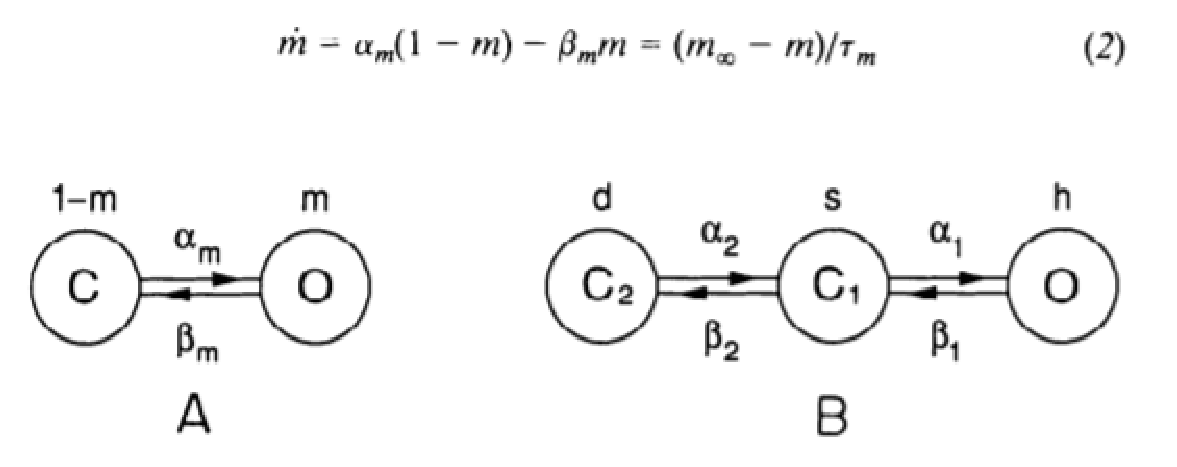
\includegraphics[height=3cm]{./images/HH-gates-T-type-Ca-Wang-1991.eps}}
  \caption{Kinetic models of T-type $\Ca$ channel: (A) an activation gate
  follows first-order kinetics; (B) the inactivtion gate has kinetics with 2 steps, i.e.
  3 states (C1 and C2 is used to account for slow recovery from inactivation
  (much slower than state transitions between C2 and O2))}
  \label{fig:HH-gates-T-type-Ca-Wang-1991}
\end{figure}


The model is then simplified using  assumption for instantaneous
(rapid) activation
\begin{equation}
I_T = \bar{g_T} s_\infty^3(\Vm) \times h \times (\Vm - E_\ca)
\end{equation}
with activation is assumed to be instantaneous, i.e. using $s_\infty$.

The current is almost fully inactivated at rest, $h \approx 0.1$ at 
$\Vm = -65$ (mV).

To elicit it, the membrane voltage must be hyperpolarized for a sufficient
amount of time in order to remove the inactivation. The current is then
activated transiently upon release from this hyperpolarized voltage level.

They have data for voltage-clamp measured at 24$^\circ$C; to test the model with
current-clamp data measured at 34-35$^\circ$C; they applied a Q10 of value 5 and
3 for activation and inactivation of T-type model, respectively. So, at body
temperature, $\tau_m$ is multiplied by 0.2; and $\tau_1, \tau_2$ are multiplied
by 0.33.


\section{T-type Ca2+ (Rush-Rinzel (1994))}
\label{sec:T-type-Ca2+-Rush-Rinzel-1994}

The model ($I_T$) for T-type $\Ca$ channel (Sect.\ref{sec:T-type-Ca2+}) was
hypothesized that voltage sensitivity of $I_T$ inactivation is increased (i.e.,
varies more steeply with voltage) - Sect.\ref{sec:Rush-Rinzel-1994}.

\begin{equation}
I_T = g_T s_\infty^3(\Vm) \times h (\Vm-E_{\rev,\Ca})
\end{equation}
where activation is assumed to be instantaneous.

The model is assumed to be almost fully inactivated at rest $h \approx 0.1$ at V
= - 65 mV).
To elicit it, the membrane voltage must be hyperpolarized for a sufficient
amount of time in order to remove the inactivation.

The current is then activated transiently upon release from this hyperpolarized
voltage level.




\section{Imredy-Yue (1994)}
\label{sec:LCC_Imredy1994}

The idea of multiple modes in gating of $\Ca$ channels
(Sect.~\ref{sec:LCC_Hess1984}) was formulated into a physical {\bf modal
switching} model by \citep{imredy1994mcs} with 2 modes. The biological mechanism
of where $\Ca$ binds to inactivate was unclear ($\Ca$ channel pore, or a domain
around the cytoplasmic entrance of the channel, or a shell underneath the
surface membranex) at that time (Sect.\ref{sec:LCC_activation_inactivation}).
[\textcolor{red}{NOTE: Nowadays, we know that calcium binds to calmodulin to
activate the inhibition.}]

\subsection{Analysis}

Different possible schemes for gating of LCC is given in
Fig.\ref{fig:Imredy_LCC}, yet only scheme IV is accepted. To study
$\Ca$-dependent inactivation, a double-pulse protocol was used. The prepulse to
induce high calcium in the cytosolic side, and then use the data at the second
pulse which give the behavior under $\Ca$-dependent inactivation.

The time to first opening (first latency) in depolarization is shorter than time
to opening after a prepulse to induce $\Ca$-sensitive inactivation. So,
$\Ca$-inactivation promote a conformation of endured closed conformation. After
the prepulse, the rise has the fast component and then a slow component of time
scale $\approx$ 100 ms. The hypothesis is that the channel can occupy a
long-lived closed state after $\Ca$ entry. So, scheme I is rejected
 
\begin{figure}[hbt]
      \centerline{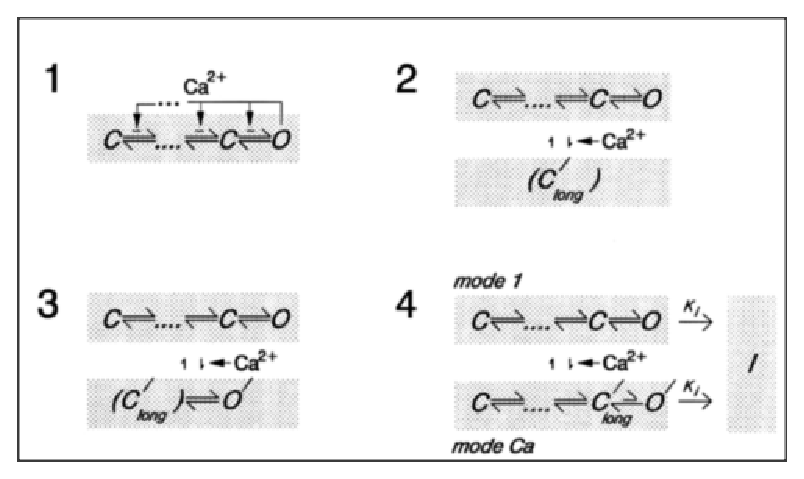
\includegraphics[height=5cm,
    angle=0]{./images/Imredy_models.eps}}
  \caption{Different schemes. Shaded areas can include multiple states
  constituting a mode. ``I'' = inactivated states underlying $V_m$-sensitive inactivation}
\label{fig:Imredy_LCC}
\end{figure}

% Also, $V_m$-sensitive inactivation also reduces channel availability which is
% typically represented by a linear activation scheme. The slow and fast
% components of the rise of channel openings excludes the kinetics picture
% represented in scheme I.  

\citep{imredy1994mcs} suggested that there should be 2 pathways leading to
opening, e.g. a long-lived closed state C'$_\text{long}$, as a side branch for
the normal pathway, to drive the slow component. However, scheme II failed to
show any apreciable change in $P_{oo}$ (the conditional probability described in
Sect.\ref{sec:keizer-maki1992}). Thus, we need a second open state O' to which
the channels in C$_\text{long}$ group can open, and the closing rate from O' is
faster than from O. The opening state O' is unstable. It's represented in Scheme
III.

Experimental results also shown that the Voltage-sensitive inactivation and
$\Ca$-inactivation are two independent processes \citep{hadley1991}.
$[\Ca]$-sensitive inactivation reduces the overall availability of a channel to
open at all. This is represented in scheme IV which is a specific subtype of
scheme III. The $\Ca$-dependent inactivation shows a discrete shift in the
pattern of gating from mode 1 (characterized by dense burst or high  $P_O$), to
mode 2 (mode $\Ca$ - characterized by infrequent  openings).
\citep{imredy1994mcs} also suggested that \textcolor{red}{there is about
100-fold reduction in the final opening rate of mode \ce{Ca^2}}.

\begin{figure}[hbt]
 \centerline{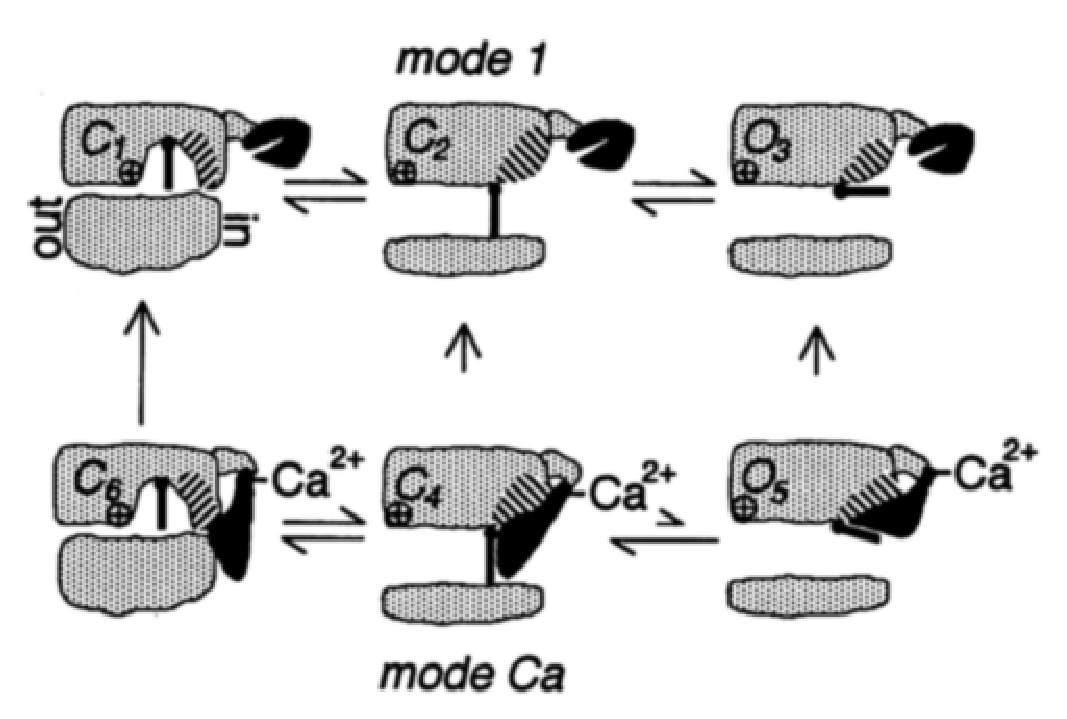
\includegraphics[height=4cm,
   angle=0]{./images/Imredy-Yue_mode.eps},
   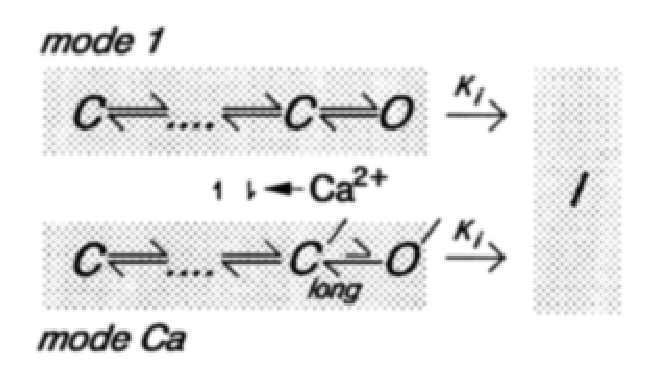
\includegraphics[height=3cm, angle=0]{./images/Imredy-Yue_LCC.eps}}
 \caption{Imredy-Yue proposed model. Mode 1 has more and long
   openings, Mode 2 or mode Ca($\ca$ sensitive inactivation) has less
   and short opening}
\label{fig:Imredy-Yue}
\end{figure}

\subsection{Proposed model}

In Fig.~\ref{fig:Imredy-Yue}, the transition $\ce{C2 <=> O3}$ is
$V_m$-insensitive. The transition rate from mode 1 to mode $\Ca$ require
a slow intermodal transition rate $K_{lu}, K_{lu}$, a function of
$V_m$. 
\begin{itemize}
\item $K_{ul} \le .025$ ms$^{-1}$
\item $K_{lu} \le .01$ ms$^{-1}$
\end{itemize}
The transition rate from mode $\Ca$ to mode 1 is state-dependent,
e.g. more rapid with \ce{C6} than with \ce{C4} than with \ce{O5}.

\begin{framed}
  
  Structurally, there are two potential evidences of
  $\Ca$-binding sites: (1) a motif resembling the EF-hand in the
  proximal C terminus; (2) an ultra-negative locus between domain 2
  and 3.
\end{framed}

However, they didn't derive any set of parameters for the gating rate constants.
Instead, they suggested that the recovery from mode $\Ca$ need to be tested over
a broad range of $V_m$, using parameters obtained from fits of the {\it first
latency distribution} F (sum of two exponential distributions)
\begin{equation}
  \label{eq:866}
  F = g \left[ f(1-e^{-t/\tau_{fast}}) + (1-f) (1-e^{-t/\tau_{slow}}) \right]
\end{equation}
where $g$ represents the plateau level of F, and $f$ is the amplitude
of the fast exponential component. $g$ provides a good measure of channel
availability at the beginning of the testpulse. F is derived from first opening
events. $f$ gauges the probability that an available channel is in mode 1 at the
beginning of the test pulse. 

With mode 1 and mode $\Ca$ are treated as two independent gating subsystems, the
opening probability
\begin{equation}
P_\text{oo,observed} = fP_\text{oo,1}+(1-f)P_\text{oo, Ca}
\end{equation}
with $P_\text{oo,1}$ and $P_\text{oo, Ca}$ are calculated from mode 1 and mode
$\Ca$ in isolation.


\section{Jafri et al. (1998) - single channel}
\label{sec:LCC_Jafri1998}

~\citep{imredy1994mcs} proposed a model in which the LCC has two modes: {\it
normal mode} and {\it calcium mode} (Sect.~\ref{sec:LCC_Imredy1994}). The
channel switches from {\it normal mode} to $\Ca$ {\it mode} when a $\Ca$ bind to
the EF-motif. In $\Ca$ mode, the channel has a much lower probability of
opening. This is essentialy similar to what suggested by \citep{marks1992}
(Sect.\ref{sec:DHPR_Marks1992}) and \citep{hess1984}.

\citep{jafri1998cad} extended this concept with a 12-state model for LCC (JRW
model), with 6 states in each mode, Fig.~\ref{fig:Jafri_mode}
(Sect.~\ref{sec:jafri-rice-winslow}).

%  \begin{figure}[hbt]
%   \centerline{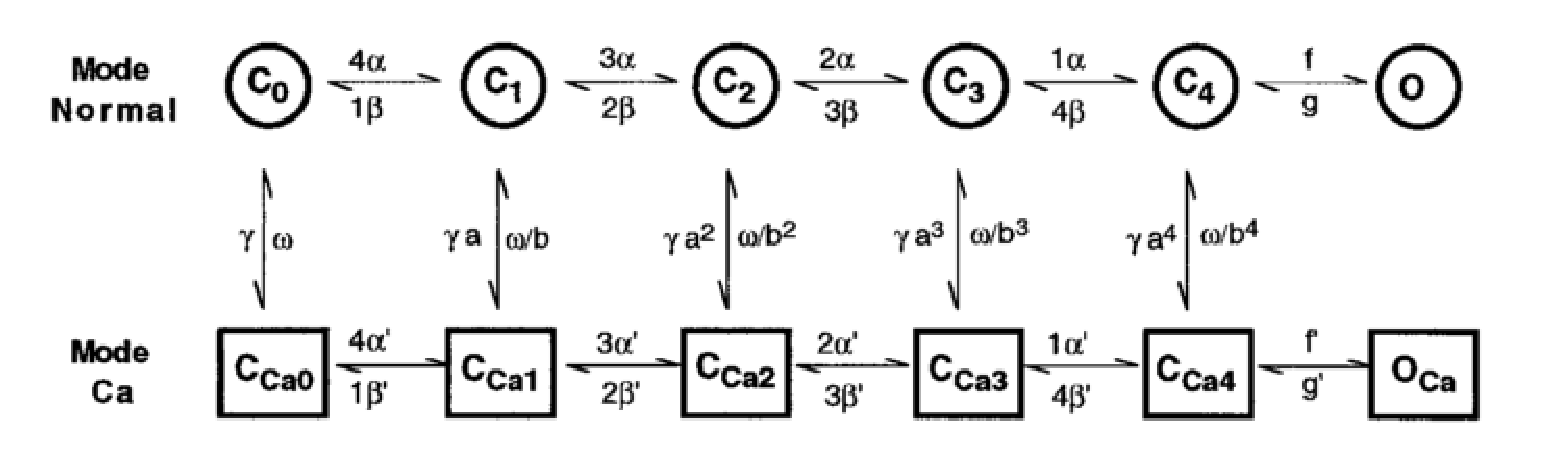
\includegraphics[height=3cm,
%     angle=0]{./images/jafri_12st_LCC.eps}}
%   \caption{2 modes, each mode with 6 states}
% \label{fig:}
% \end{figure}

% Experimental data suggested the importance of $\Ca$-binding inactivation of LCC
% \citep{deleon1995ecb} (Sect.\ref{sec:LCC_activation_inactivation}). However, in
% early models, $\Ca$-inactivation of $\Ca$-channel was represented using a
% Michaelis-Menten-type function, which assume instantaneous inactivation or
% activation after $[\ca]_i$ elevation or $[\ca]_i$ falls, respectively. As there
% were evidences of time-dependent inactivation. 
% 

\begin{figure}[hbt]
  \centerline{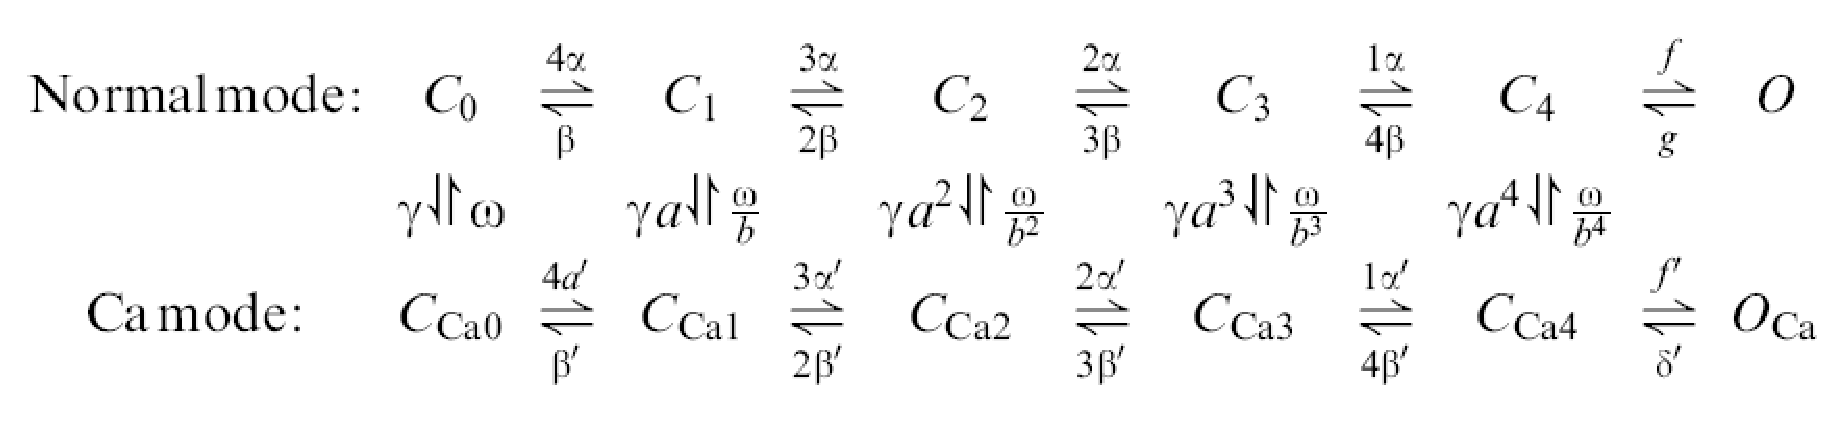
\includegraphics[height=2.7cm,
    angle=0]{./images/Jafri_mode_switching.eps}}
  \caption{Switching between two modes: Normal vs. Calcium-dependent}
  \label{fig:Jafri_mode}
\end{figure}

The choice of 6 states in each mode is based on the fact that the ionic channel
is tetrameric with 4 subunits and the assumption that the activation requires
the sequential binding of 4 agonists, each to a subunit. The subunits are
assumed to be identical, so that an agonist can bind to any of them. The
switching between 2 neighboring states is represented via gating variables
\begin{itemize}
\item $V_m$-dependent activation gating variable for each subunit is
  $\alpha$ (increase with $V_m$). Example: at state $C_0$ there are 4
  available subunits, then the probability for the binding to occur is
  $4\alpha$.

\item $V_m$-dependent inactivation gating variable for each subunit is
  $\beta$ (decrease with $V_m$). 
\end{itemize}
$\Ca$-dependent inactivation is modeled as mode-switching with the transition
rate is a function of $[\Ca]$.


\begin{framed}
  The close symmetry between the two modes and similarity of rates are
  due to the fact that gating currents in experimental data are very
  similar between the two modes \citep{hadley1991, shirokov1993cdi}, and also to
  avoid explosion of parameters to estimated.
\end{framed}

A single subunit transition between closed and open conformation are
$V_m$-dependent, and the rate constants follow the first-order reaction
where the rate is an exponential function of $V_m$ ({\it general law})
\begin{equation}
\begin{split}
\alpha = \alpha_0 \times \exp\left( \alpha_1 . (V_m - V_0) \right) \\
\beta = \beta_0 \times \exp \left( \beta_1 . (V_m - V_0) \right)
\end{split}
\end{equation}


In addition, in JRW model, the inactivation is by $[\ca]_\ds$ (ds
= dyadic subspace)\footnote{original paper use $[\ca]_{ss}$} which
is higher than $[\ca]_i$. So, the affect of calcium-inactivation
is the fast component while $V_m$-dependent inactivation is the slow component.

The higher the membrane potential $V_m$, the more $[\ca]_\ds$ to
be released, thus increasing the probability of switching to
$\Ca$ mode. Thus, at state $C_3$, it's more likely to switch to
Ca-mode than at state $C_1$ and $C_2$. To model this, the elementary
transition to $\Ca$ mode $\gamma$ is multiplied to a factor
$a>1$, each time the state index is higher. Along with that, the
transition rate from $\Ca$ mode to normal mode would decrease,
which is modeled as the divisor on $\omega$ by a factor $b>1$. 

Using deterministic approach, $C_i, C_{\ca i} (i=1...4)$ represent the fraction
of LCC channels in each closed state. Each LCC is composed of 4 subunits whose rate
transition between activation and inactivation are considered as
atomic events, i.e. fixed rate transitions. For example: in normal
mode, the rate transition from inactive to active for a single subunit
is $\alpha$. At $C_0$, with 4 inactivated subunits, the probability
for $C_0$ to have one activated subunit is $4\alpha$.

Here, there are two open states: $O$ and $O_\ca $. The transition to
these two states are controlled by two $V_m$-independent rate constant
$f$ and $f'$ in which $f'$ is 500 times smaller than $f$.  
\begin{itemize}
\item The change in the fraction of LCC in each state is denoted by
  ODEs, as given in eq.~\eqref{eq:777}.

\item Mathematical description for the elementary transition rates is
  given in eq.~\eqref{eq:763}.
\end{itemize}

\begin{framed}
  REMEMBER: when designing a Markov chain model:
  {\it micro reversibility} requires that for each (closed) cycle, the
  product of transition rates in one direction is equal to the product
  of transition rates in the other direction.
\end{framed}

LCC is assumed to permeate only $\Ca$ (inward) and $\K$ (outward). The
permeation through the channel is modeled using constant-field theory where
permeability of $\K$ is modified as a decreasing function of $\Ca$ current,
eq.\ref{eq:780}.

\begin{figure}[hbt]
  \centerline{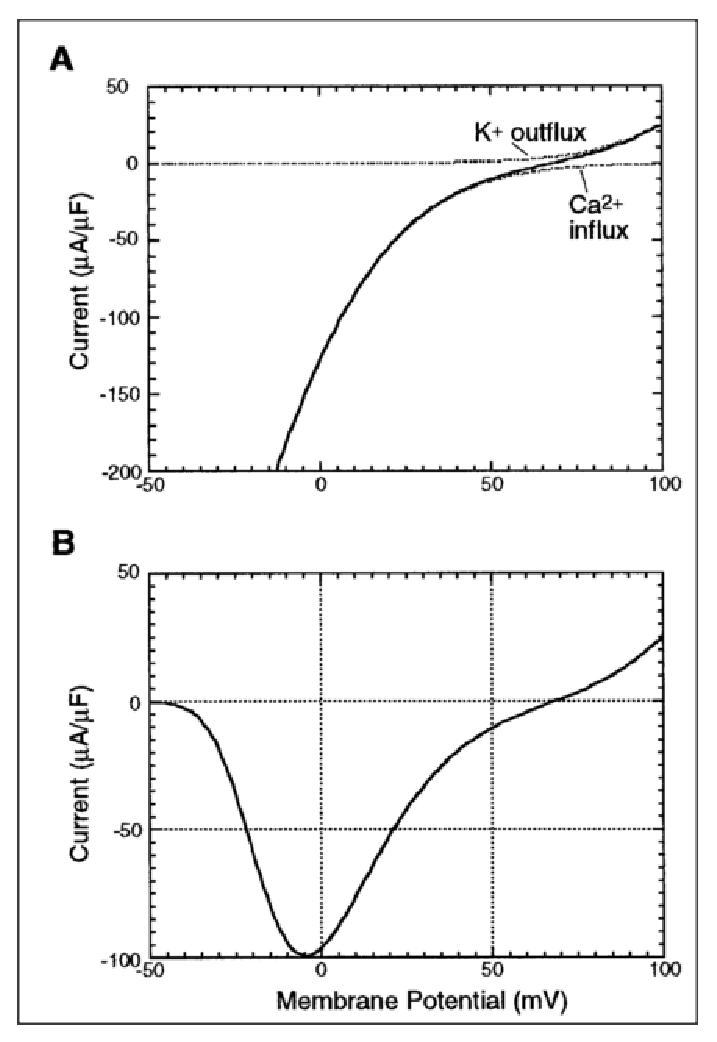
\includegraphics[height=5cm,
    angle=0]{./images/Jafri_98_LCC-current.eps}}
  \caption{(A) I-V relation for an open LCC (solid line: permeation model,
  dashed line: separate contribution by $\Ca$ and $\K$); (B) Peak $I_\ca$ is
  obtained by multiplying the open LCC I-V relation above with $P_{o,\max}$}
  \label{fig:Jafri98_LCCcurrent}
\end{figure}


The I-V relation of the model is multiplied by $P_o$ to simulate $V_m$-clamp
data, Fig.\ref{fig:Jafri98_LCCcurrent}, and fitted to experimental data from
\citep{mcdonald1986}. However, the major problem is that there are too many
states, and thus many parameters to be fitted. As a result, there can be many
parameter sets can fit the experimental data.
% However, $V_m$ inactivation has not been considered yet.
% \citep{stern1999lcm,greenstein2002} incorporated $V_m$-dependent inactivation
% (Sect.~\ref{sec:LCC_stern1999}, \ref{sec:greenst-winsl-2002}).

\section{Stern et al. (1999)}
\label{sec:LCC_stern1999}

\citep{stern1999lcm} proposed 24-state gating scheme for LCC. The
scheme has 4 modes (mode 1, mode Ca, mode 2 (or mode V), and mode
Ca-V), more than Jafri et al. 12 states model, as $V_m$ inactivation
is incorporated as a different mode. Each mode with a cascade of 5 closed state,
connected by 4 gating variables, and one last open state.

\begin{figure}[hbt]
  \centerline{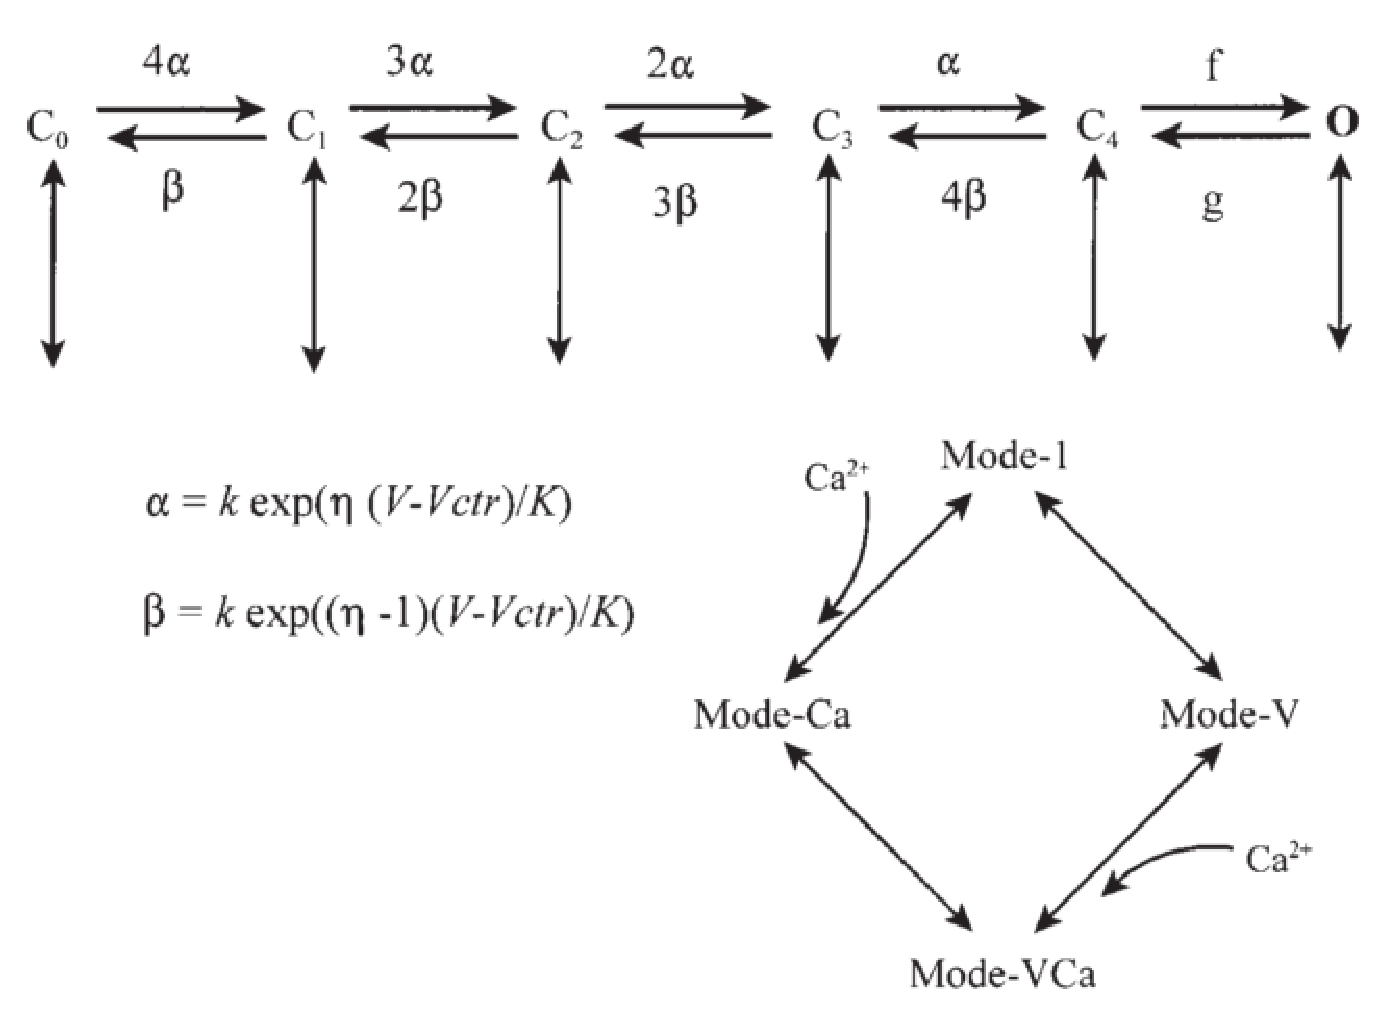
\includegraphics[height=5cm,
    angle=0]{./images/Stern_24st_LCC.eps}}
  \caption{5 modes, each mode with 6 states, having similar state
    transitions, with opening in the rightmost state}
\label{fig:Stern_24stateLCC}
\end{figure}


LCC is believed to be both $V_m$ inactivation and $\ca$ inactivation. So, in
mode-Ca, the binding of $\ca$ may inhibit the activity of the channel. Similar
to mode-$V_m$, which shift the activation potential to the left. The data shown
I-V curve has bell-shaped and the channel activate the most at between 0 - 20
mV, i.e. peak $I_\dhpr$ reaches the maximum in this range. However, the model is
not widely used due to its high number of state that may lead to high
computational expensive.

\section{Sun et al. (2000) - rat }
\label{sec:LCC_Sun2000}

\begin{framed}
Modal switching models are high-order, with so many parameters to fit.
Hodgkin-Huxley-based models are lower-order, more compact approximation; yet
many not be able to adequately characterize the complex dynamics of ion 
channels.  An alternate is to use a lumped {\bf multiple-state model} with
Markovian characteristics. 
  
\end{framed}

\begin{figure}[hbt]
  \centerline{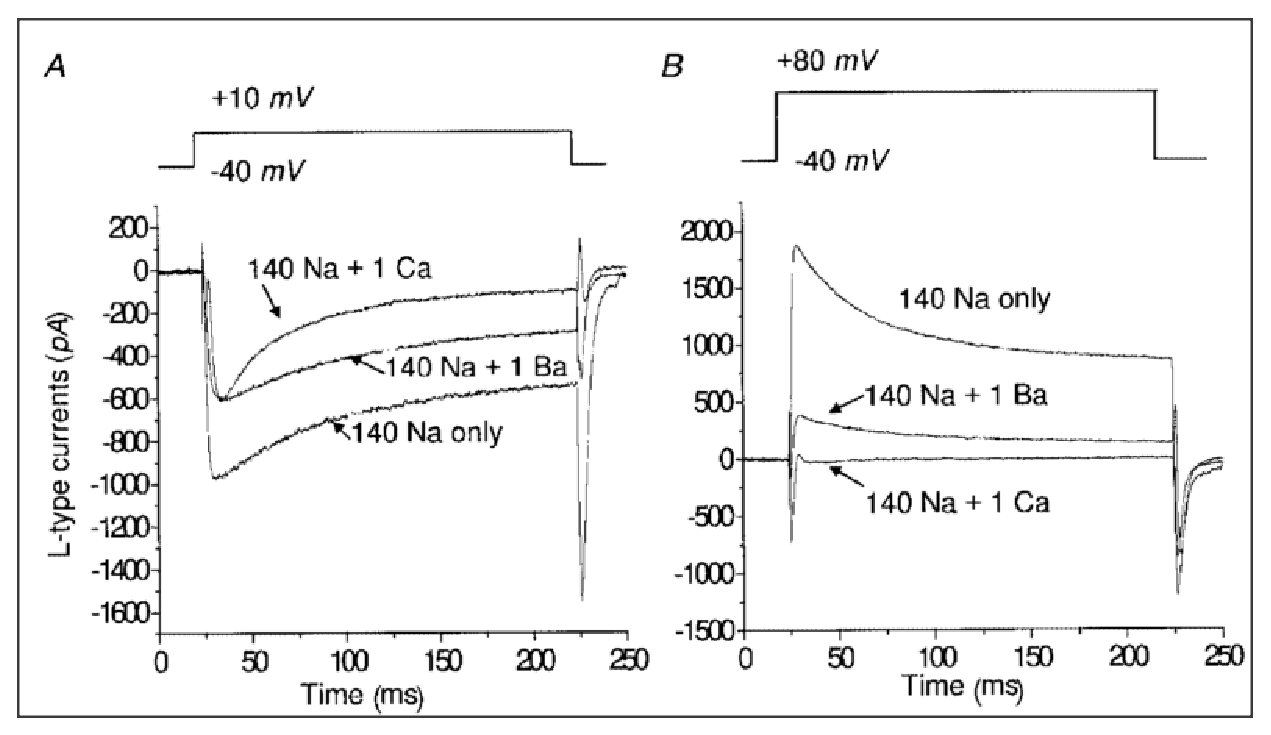
\includegraphics[height=5cm,
    angle=0]{./images/Sun_experiment_1.eps}}
\centerline{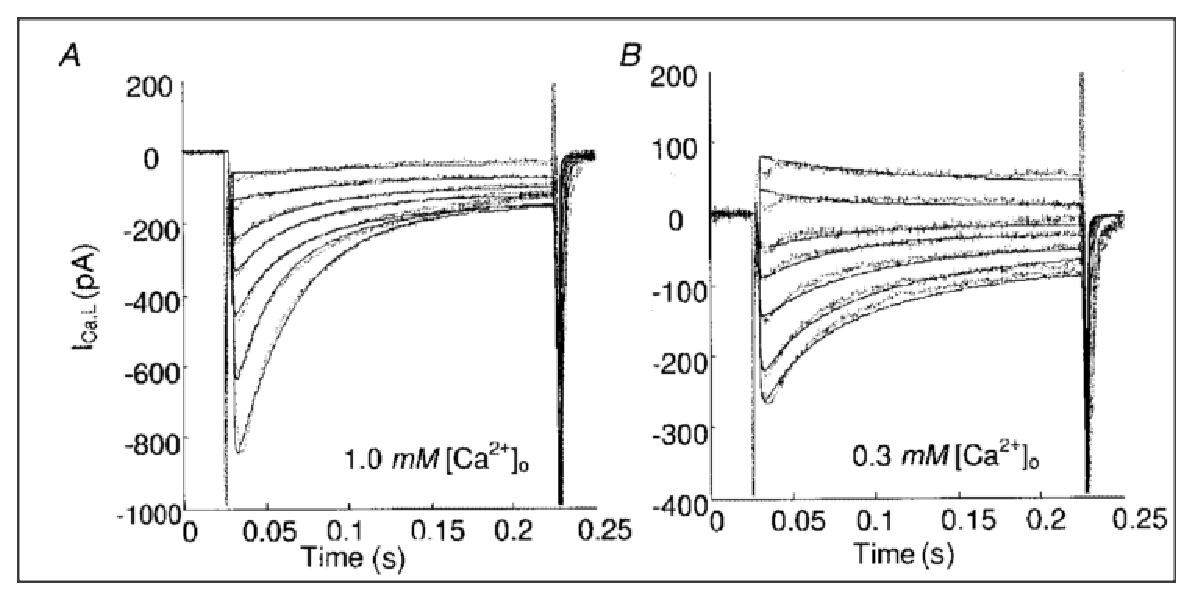
\includegraphics[height=5cm,
    angle=0]{./images/Sun_experiment_2.eps}}    
\caption{First pair: Holding potential -40 mV; labels are extracellular
concentration (mM). (A) step potential +10mV, (B) +80mV. In the second pair:
voltage-clamp data using different $[\Ca]_o$}
\label{fig:Sun_Ica}
\end{figure}

\citep{sun2000mlc} developed LCC that assumes to permeate different ions $\Ca$,
$\Ba$, $\Na$, and $\Cs$ (multi-ion single-file channel containing at least two
ion binding sites) \citep{hess1984}. Extracellular calcium bind to the
allosteric high-affinity regulatory site in a voltage-dependent fashion to
convert the channel into monovalent-impermeant state. The first component in
the following equation reflects the effect of blocking $i_\na, i_\cs$ at high
$[\Ca]_o$ (or $[\Ba]_o$). At low $[\Ca]_o$, the divalent cations produce less
current than the monovalent. However, at high $[\Ca]_o$, it boost $\Ca$ inward
currents. This U-shaped $[\Ca]_o$ dependence is simulated macroscopically by
introducing a $[\Ca]_o$-dependent repulsion function in front of the $i_\ca$
term. Fig.\ref{fig:Sun_Ica} shows current data.

In essence, depending upon which divalent ions is being used in the bathing
medium, the expression for total current across LCC are given as

\begin{equation}
\begin{split}
i_\tot = i_{\Ba,\tot} = \frac{K_\ba(V_m)}{K_\ba(V_m)+[\Ba]_o)} (\overline{i_\na} +
\overline{i_\cs}) + \\
\left( \frac{-1}{1+ \exp\left( ([\Ba]_o - 0.08)/0.00159 \right)} +1 \right)
i_\ba
\end{split}
\end{equation}
or
\begin{equation}
\begin{split}
i_\tot = i_{\Ca,\tot} = \frac{K_\ca(V_m)}{K_\ca(V_m)+[\Ca]_o)} (\overline{i_\na} +
\overline{i_\cs}) +
\\
\left( \frac{-1}{1+ \exp\left( ([\Ca]_o - 0.08)/0.00159 \right)} +1 \right)
i_\ca
\end{split}
\end{equation}

The microscopic total unitary current going through a single opening channel is
$i_\tot$, with $K_\ba(V_m)$ and $K_\ca(V_m)$ are voltage-dependent binding
function of divalent ions; $\overline{i_\na}, \overline{i_\cs}$ are the maximum of the
corresponding current component through a single open channel for $\Na$ and
$\Cs$, respectively.
\begin{eqnarray}
K_\ba(V_m) = 0.00132\exp\left( (V_m-21.73)/21.24 \right) \\
K_\ca(V_m) = 0.00105\exp\left( (V_m-21.73)/21.24 \right) 
\end{eqnarray}

\begin{figure}[hbt]
 \centerline{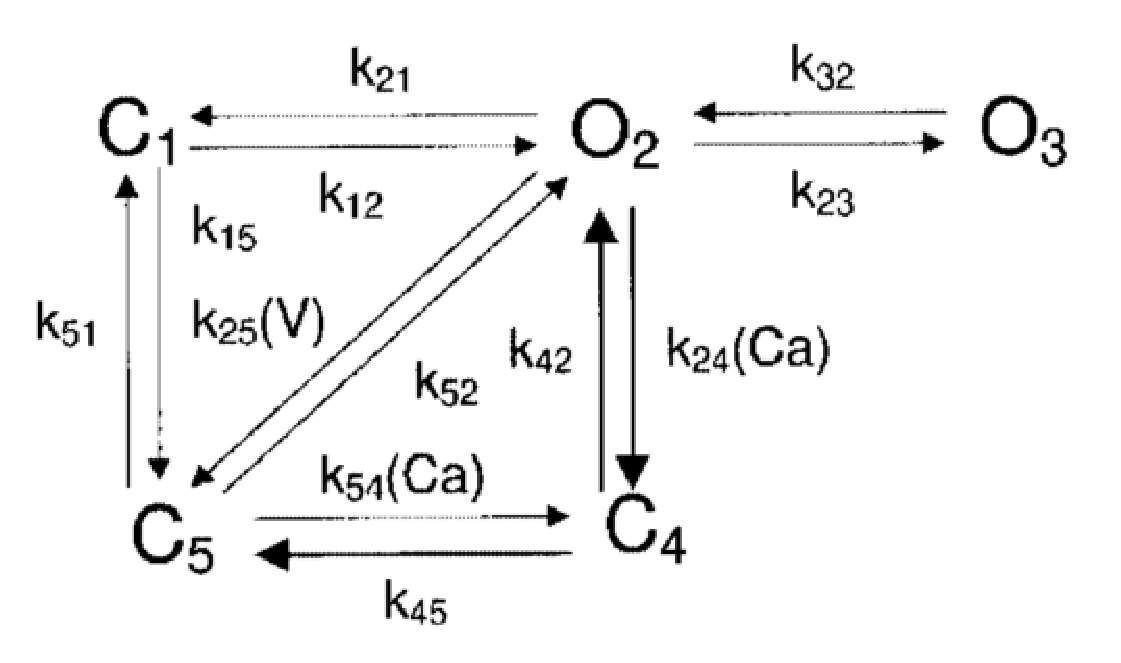
\includegraphics[height=5cm, angle=0]{./images/Sun_DHPR.eps}}
\caption{Schematic diagram of L-type channel. $k_{24}, k_{54}$ are
Calcium/Calmodulin dependent}
\label{fig:Sun_DHPR}
\end{figure}

GHK equation (Sect.\ref{sec:GHK_voltage}) is used to represent
microscopic individual ionic current via a single L-type $\Ca$ channel
\begin{equation}
\begin{split}
i_\na &= P_\na .z_\na^2 \left( \frac{VF^2}{RT}\right) \left( \frac{0.75
[\Na]_i e^{VF/RT} - 0.75 [\Na]_o}{e^{VF/RT} - 1} \right) \\
i_\cs &= P_\cs .z_\cs^2 \left( \frac{VF^2}{RT}\right) \left( \frac{0.75
[\Cs]_i e^{VF/RT} - 0.75 [\Cs]_o}{e^{VF/RT} - 1} \right) \\ 
i_\ca &= P_\ca .z_\ca^2 \left( \frac{VF^2}{RT}\right) \left( \frac{
[\Ca]_i e^{VF/RT} - 0.341 [\Ca]_o}{e^{VF/RT} - 1} \right) \\ 
i_\ba &= P_\ba .z_\ba^2 \left( \frac{VF^2}{RT}\right) \left( \frac{
[\Ba]_i e^{VF/RT} - 0.341 [\Ba]_o}{e^{VF/RT} - 1} \right) \\ 
\end{split} 
\end{equation}
with the permeability $P_Y=(D_Y.\beta_i)/l$. 
\begin{itemize}
  \item $P_\na=8.0355\times 10^{-5}$
  \item $P_\cs=6.2088\times 10^{-5}$
  \item $P_\ca=67.367\times 10^{-4}$
  \item $P_\ba=41.456\times 10^{-4}$ 
\end{itemize}
and $[\Na]_o=140.0$ (mM), $[\Cs]_o=3.0$ (mM), $[\Cs]_i=140.0$ (mM).

The diffusion constant $D(x)$ is constant in \ce{Na+}, \ce{Ca^2+}, \ce{Ba^2+}
cases; and in the case of \ce{Cs+}, it's a function
\begin{equation}
  \label{eq:868}
  D(x) = \overline{D} e^{\frac{2z_YFV_m(L-x)}{RT}}
\end{equation}
NOTE: $\beta_o=\beta_i=0.75$ for $\Na$ and $\Cs$; $\beta_o=0.341; \beta_1=1.0$
for $\Ca$ and $\Ba$.

\citep{sun2000mlc} modeled the L-type $\Ca$ channel with 5 states,
Fig.~\ref{fig:Sun_DHPR}. The LCC-model has both voltage-dependent and
calcium-dependent inactivation. The transition rates are determined only by the
initial states and by external variables, e.g. membrane potential and $[\Ca]$.
\begin{enumerate}
  \item At resting, the channel is at closed state C$_1$. 
  \item Under depolarization, the channel quickly open, switching to open state
  O$_2$. 
  \item The inactivation is complex with 2 independent pathways: $V_m$-dependent
  (O$_2$ to C$_5$) and $[\Ca]$-dependent (O$_2$ to C$_4$ and then to C$_5$). 
\begin{equation}
  \label{eq:867}
  \begin{split}
    \ce{O2 &<=>[\Ca] C4 <=> C5 } \;\; ; \text{both fast \& slow
      phase $\Ca$ inactivation}\\
    \ce{O2 &<=>[V_m] C5 }
  \end{split} 
\end{equation}
  
  So, $I_\CaL$ declines with 2 component time courses. The fast component is
  seemd to be $[\Ca]$-dependent, and the slow one is both $\Ca$-independent and
  $V_m$-dependent. To model this fast component, an intermediate closing state
  C$_4$ is used. To model the slow component, a common C$_5$ state is used.
  These two separate and distinct decay processes are a fundamental assumption
  in other models as wells (Sect.\ref{sec:LCC_Imredy1994}, .\ref{sec:LCC_Jafri1998}).
   
   \item The pathway connecting C$_5$ and C$_1$ characterize the
   so-called ``ultra-slow'' inactivation process \citep{boyett1994}. This
   pathway is masked by $\Ca$-dependent inactivation and $\Ca$-dependent
   inactivation. However, if the duration of the conditioning pulse is long
   enough, e.g. 20s, it can manifest itself. [NOTE: We thus can merge C5 and C1
   if we don't consider long pulse. In such case, we need to modify the rate
   constants accodingly].
    
    \item The additional open state $O_3$ represent the long-lasting open
    channel state to account for the increased tail current at large
    depolarization ($V_m> +40$mV).

{\bf Tail current}: A long-lasting open channel state $O_3$ is added which is a
lumped state of 2 ditinct gating pattern described by \citep{pietrobon1990}. At
small $V_m$, $k_{23}$ is very small, and will become significant only at very
large and long $V_m$.

    \textcolor{red}{It's assumed single channel conductance is the same at two
    open state O$_2$ and O$_3$}.
\end{enumerate}

Then, the whole-cell current for $N$ LCC channels is
\begin{equation}
I_\CaL = N \times i_\tot \times (P_{O2}+P_{O3})
\end{equation}

\subsection{Parameter estimation}

{\bf Rate constants} (transition rates): they are all measured at steady-state
condition. There are two open states O2 and O3. The transition from O2 to O3 is
voltage-independent and represent the steady-state open probability.

When the two different pathways are masked to each other, we need to follow
different experimental conditions to find individual pathway separatedly. An
example is there are two inactivation pathways, in order to measure the rate
constants, say voltage-dependent inactivation $k_{21}$, all other factors need
to be controlled, e.g. NOT using $\Ca$ as charge carriers.

\begin{enumerate}
  \item $V_m$-depenent activation: $\ce{C1 <=>[k_{12}(V_m)][k_{21}(V_m)] O2}$.
  
  As the time constant for the activation is much faster ($\ge 100$ times) than
  those of inactivation kinetics, so they reasonably assume that when the
  activation occurs, there is no channel in states other than C$_1$ and
  O$_2$. So $P_{C1}+P_{O2}=1$, and
  \begin{equation}
  dP_{C1}/dt = k_{21}P_{O2} - k_{12}P_{C1} \;\;; dP_{O2}/dt =
  k_{12}P_{C1}-k_{21}P_{O2}
  \end{equation}
Using the approach of Sect.\ref{sec:model-ion-channel}, a single function in
which the change in fraction of channels in $O_2$ can be written in the form of
steady-state activation $P_{O2,\infty} (V_m)$ and activation time constant
$\tau_{O2,\infty} (V_m)$ (both are function of $V_m$).
\begin{equation}
dP_{O2}/dt = \frac{P_{O2,\infty}(V_m)-P_{O2}}{\tau_{O2,\infty}}
\end{equation}
with 
\begin{equation}
P_{O2,\infty}(V_m)=\frac{k_{12}(V_m)}{k_{12}(V_m)+k_{21}(V_m)} \;\;; 
\tau_{O2,\infty}(V_m)=\frac{1}{k_{12}(V_m)+k_{21}(V_m)} 
\end{equation}
From this, we can reverse the equation to find $k_{12}$ and $k_{21}$.
\begin{equation*}
k_{12}(V_m)=\frac{P_{O2,\infty}(V_m)}{\tau_{O2,\infty}(V_m)} \;\;;
k_{21}(V_m)=\frac{1-P_{O2,\infty}(V_m)}{\tau_{O2,\infty}(V_m)} 
\end{equation*}

NOTICE: After incorporating other states (particularly voltage-dependent
inactivation states), the system need to be adjusted so that the opening
probability $P_O$ should be in the range 0.3-0.7 at +10 mV to +60 mV
depolarization \citep{cachelin1983}. Then, an new factor \verb!att! is added to
$k_{12}$.
\begin{equation}
\att = \frac{-4867.42}{1+\exp^{(V_m-35.0)/3.53}} +
\frac{-130.5}{1+\exp^{(V_m-10.574)/0.89}} + 4998.92
\end{equation}
\begin{equation}
k_{12}(V_m)=\frac{P_{O2,\infty}(V_m)}{\tau_{O2,\infty}(V_m)} \att \;\;;
k_{21}(V_m)=\frac{1-P_{O2,\infty}(V_m)}{\tau_{O2,\infty}(V_m)} 
\end{equation}

Here, steady-state $P_{O2,\infty}$ and $\tau_{O2,\infty}$ are estimated from
voltage-clamp experimental data by fitting a Boltzmann distribution (sigmoidal
kinetisc), and the sum of two Gaussian functions, respectively,
Fig.\ref{fig:Sun_activation}. 

\begin{figure}[hbt]
 \centerline{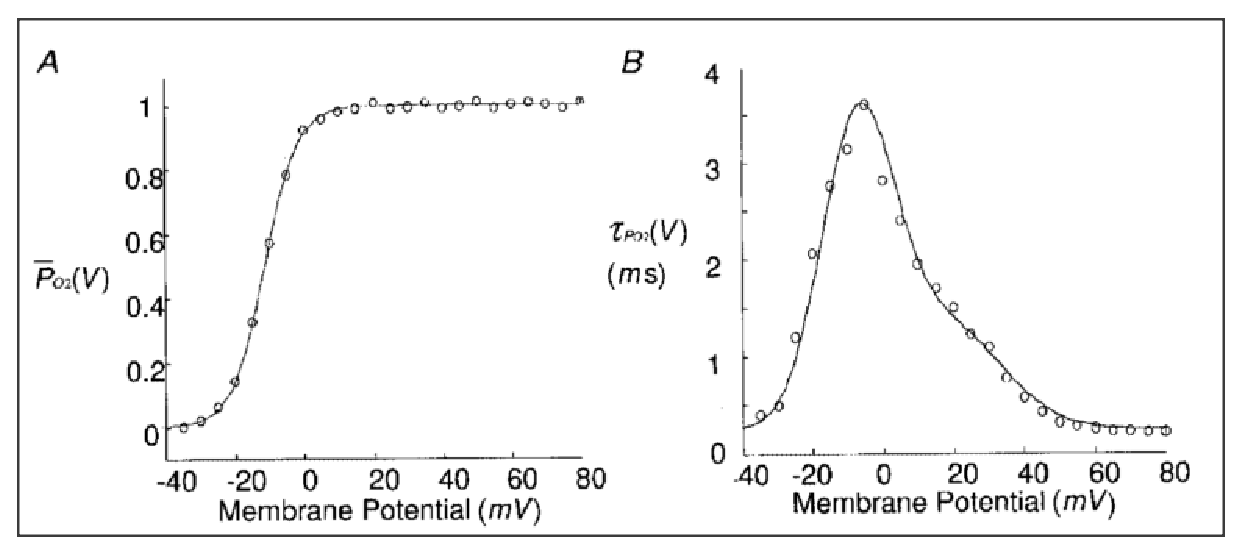
\includegraphics[height=5cm]{./images/Sun_activation.eps}}
\caption{Activation: steady-state fraction of opening channels $P_{O2,\infty}$
and time constant $\tau_{O2,\infty}$}
\label{fig:Sun_activation}
\end{figure}

The general forms for steady-state opening probability
\begin{equation}
P_{O2,\infty}(V_m)= \frac{-1.0}{1.0+\exp\left(\frac{V_m-V_{1/2}}{S}\right) } +
1.0
\end{equation}
with $V_{1/2}$ is the activation threshold which can be adjusted by changing the
extracellular $\Ca$ (or $\Ba$), $S$ is related to the inverse slope of the
activation curve at $V_{1/2}$.

Experimental data also showed a small increase in $[\Ca]_o$ (still in the range
0.0 - 1.0 mM), can shift the voltage activation threshold $V_{1/2}$ from -28.6
mV to -11.4 mV. This positive-directive shifting effect saturates at $[\Ca]_o=40$ mM
\citep{kwan1993}. So, to characterize this shifting, an equation that fits
well to $[\Ca]_o-V_{1/2}$ data (least-square fit) is
\begin{equation}
V_{1/2} = -16.334 + 13.31 \exp\left(-[\Ca]_o/0.053 \right) + 31.65 \exp\left(
-[\Ca]_o/11.305 \right)
\end{equation}
and 
\begin{equation}
S = \left(0.632 + 0.368 \exp(\frac{-([\Ca]_o-0.1)}{0.784})\right)
\frac{-3.792}{1 + \exp\left( \frac{[\Ca]_o - 0.0469}{0.011}\right)} +
3.695
\end{equation}

\begin{equation}
\tau_{O2,\infty}(V_m) = 0.00025 + 0.00305 \exp(-0.0045(V_m+7.0)^2) + 0.00105
\exp(-0.002(V_m-18.0)^2)
\end{equation}


\item $V_m$-dependent inactivation: To avoid the effect of $\Ca$ or
$\Ba$-dependent inactivation, ionic substitution experiments were carried out
where $\Na$ or $\Cs$ are charge carriers via L-type $\Ca$ channels, i.e.
$[\Na]_o=$140 mM (no $\Ca_o,\Ba_o$), $[\Cs]_i=$140 mM.

They need a good initial guess for $k_{25}(V)$ and $k_{52}(V)$ by using
the strategy below. The authors ignored the effect of $V_m$-dependent activation
and the transition from $O_2$ to $O_3$, so the two transition rates
$k_{25}(V_m)$ and $k_{52}(V_m)$ are estimated from the two-state scheme:
 $\ce{O2 <=>[k_{25}(V_m)][k_{52}(V_m)] C5}$.

Again, they need to estimate the steady-state $P_{O5}(V), \tau_{O5}(V)$. The
time course inactivation need to be determined using double-pulse protocol with
100ms interval in between. Based on the corresponding experimental data,
Fig.\ref{fig:Sun_inactivation}, they suggested each one should be expressed as
the sum of two Boltzmann functions (i.e. combine of two sigmoidal curves
continuitively). 

% Remember that $k_{25}$ and $k_{52}$ obtained from the above distribution are not
% accurate since $V_m$-dependent inactivation is not completely independent of
% $V_m$-dependent inactivation and the transition from $O_2$ to $O_3$.

Definitely, when adding $k_{25}$, it reduces $P_{O2,\infty}(V)$. So, to push the
open probability of LCC to the proper range, an attenuation factor \verb!att!
was added to $k_{21}$.

\begin{figure}[hbt]
 \centerline{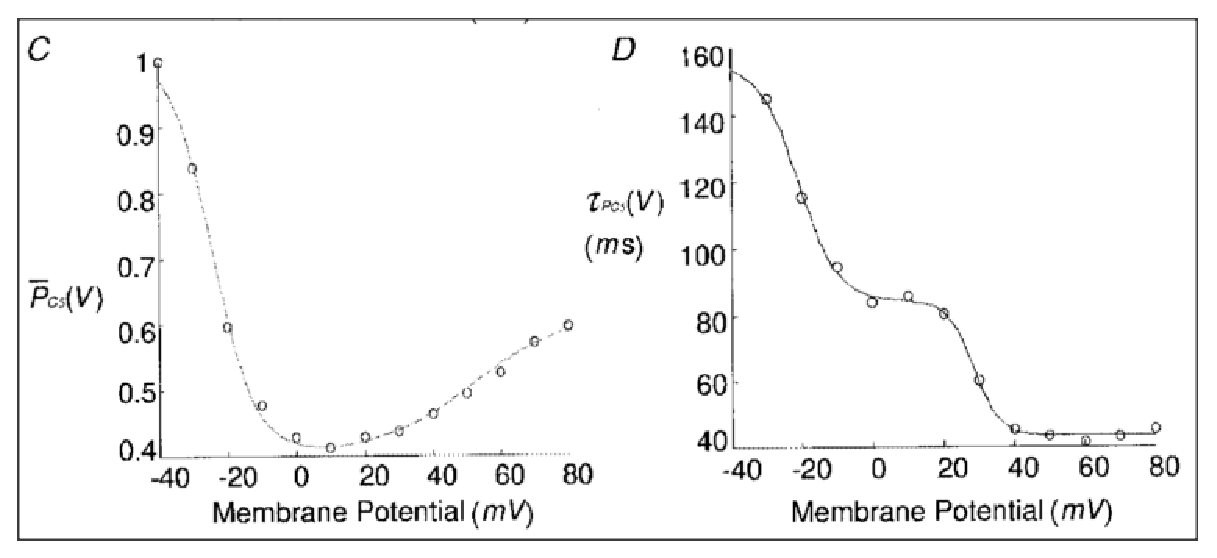
\includegraphics[height=5cm]{./images/Sun_inactivation.eps}}
\caption{Inactivation: steady-state fraction of opening channels $P_{O5,\infty}$
and time constant $\tau_{O5,\infty}$ (data obtained using two-pulse protocol
with 100ms interval in between)}
\label{fig:Sun_inactivation}
\end{figure}

Similarly, when considering $\Ca$-dependent inactivation states, it will bring
down $P_{O2,\infty}(V)$. To account for $\Ba$ and $\Ca$-dependent inactivation,
the new coefficient $k^*_{25}$ is formulated as the product of the conventional
rate coefficient and an inhibition factor \verb!(1-inh)!. NOTE: \verb!inh! rises
from 0.2 (at +40mV) to 0.9 (at +80 mV) when $[\Ca]_o=1.0$ (mM).
\begin{equation}
\begin{split}
k_{25} &= \left( \frac{-18.465}{1+\exp^{(V_m-51.23)/6.785}} + 32.0 \right) \\
k^*_{25} &= k_{25} \times (1 - \inh) \\
k_{52} &= \frac{-5.0}{1+\exp^{(V_m-30)/0.787}} + 6.0
\end{split}
\end{equation}
with the value of \verb!inh! receive the appropriate formula depending we use
$\Ca$ or $\Ba$.
\begin{eqnarray}
\inh(\Ca) &&= \left( \frac{-0.888}{1+\exp^{(V_m-43.066)/2.289}} + 0.89 \right)\\ 
&& \left( \frac{-1.199}{1+\exp^{([\Ca]_o-0.259)/0.164}} + 1.004 \right) \\
\inh(\Ba) &&= \left( \frac{-0.888}{1+\exp^{(V_m-43.066)/2.289}} + 0.89 \right)\\
&& \left( \frac{-1.199}{1+\exp^{([\Ca]_o-0.259)/0.164}} + 1.004 \right)\times
0.1
\end{eqnarray}
$\inh$ as a function of $V_m$ and $[\Ca]_o$ rise from 0.2 (at +40mV) to 0.9 (at
+80mV) when $[\Ca]_o=1.0$mM. The inhibition function increase sharply with
increasing $[\Ca]_o$, and also increase, but slower, with increase in voltage
> +20 mV. 

\item $[\Ca]_o, [\Ca]_i$-mediated inactivation: the effect of $[\Ca]_o$ is added
as a term to $i_\ca$ as described from the beginning of the section. In the case
of $[\Ca]_i$, it needs to be able (1) inactivation occurs faster at negative
potential (as $\Ca$ flux through the channel is greater at negative
depolarizations that at positive potentials), (2) the bigger the unitary
currents $i_\ca$ at negative potential, the more likely to inactivate the
channel.

As calmodulin (CMD) is the $\Ca$-sensor for $\Ca$-dependent inactivation. So,
$k_{24}$ is a function of the Ca-CMD complex
\begin{equation}
k_{24} = c_{24} [\CaCaM]_\DHPR
\end{equation}
with $c_{24}$ is a constant, and the binding of $\Ca$ to $\CaM$ depend on the
local calcium concentration with a Hill coefficient 3 \citep{qin1999}.
\begin{equation}
d[\CaCaM]_\DHPR/dt = k^+_\CaM [\Ca]_\DHPR^3 ([\CaM]_\tot - [\CaCaM]_\DHPR) -
k^-_\CaM [\CaCaM]_\DHPR
\end{equation}
Total CaM concentration and rate constants are derived from \citep{smith1998}. 

In the case of $\Ba$ as charge carriers, the inactivation is considered lower
(100x slower) compared to $\Ca$. So, when $\Ba$ is used, the model is the same,
except association constant of $\Ba$ to CaM is reduced to 10\% of that of $\Ca$. 

There are evidences that $[\Ba]_o$ and $[\Ca]_o$ also affect voltage-dependent
inactivation pathway where we don't find when $\Na$ or $\Cs$ is used as charge
carriers. So, $k_{25}$ need to be adjusted, and the new coefficient $k^*_{25}$
is used (see above). 

\item At high depolarization (> +40mV), there is a pronounced decrease in
voltage-dependent inactivation (when $[\Ca]_o=1.0$mM is used). To explain for
this, 
\end{enumerate}


The fraction of channels in each state is calcualted using ODEs
\begin{equation}
\begin{split}
dP_{C1}/dt &= k_{21} P_{O2} + k_{51} P_{C5} - (k_{12}+k_{15}) P_{C1} \\
dP_{O2}/dt &= k_{12} P_{C2} + k_{32} P_{O3} + k_{42} P_{C4} + k_{52} P_{C5} -
(k_{21}+k_{23}+k_{24}+k_{25}^*) P_{O2} \\
dP_{O3}/dt &=  \\
dP_{C4}/dt &=  \\
dP_{C5}/dt &= 
\end{split}
\end{equation}

\begin{framed}
To study the dynamics of LCC (amplitudes and dynamics), they eliminated all
$\Ca$ contribution from RyR release (by applying high dose of ryanodine
$20\muM$). Extracellular  $[\Ca]_o=1.0$ (mM) is assumed to be constant. $\Ca$
entry via LCC is assumed to diffuse passively.
\end{framed}



\subsection{Data analysis}
\label{sec:Sun_dataanalysis}

The gating of LCC is put into the context of a small restricted
subsarcolemmal space $V_c$, in addition to the extracellular $V_e$ and
intracellular volume $V_i$. The cleft space is  modeled as a narrow cylindrical
space, i.e. a dyadic subspace  with dyadic gap $h\sim 15$ (nm) and width from
60-120 nm (they use h=18nm, d=120nm), Fig.\ref{fig:Sun_DHPR_cellmodel}. The
diffusion constant of $\Ca$ ranges from 100-600 $\mum^2/s$ (they use $D_\ca=250\mum^2/s$).

Polar coordinates were used in computation. The calcium at the center (0,0) is
responsible for LCC $\Ca$ current inactivation, and the calcium at the mouth of
RyR, i.e. point (0,h), is responsible for RyR $\Ca$ activation and inactivation.
The boundary condition at r=d/2 for local $[\Ca]_\ds$ is the cytosolic
$[\Ca]_i$.

\begin{figure}[hbt]
 \centerline{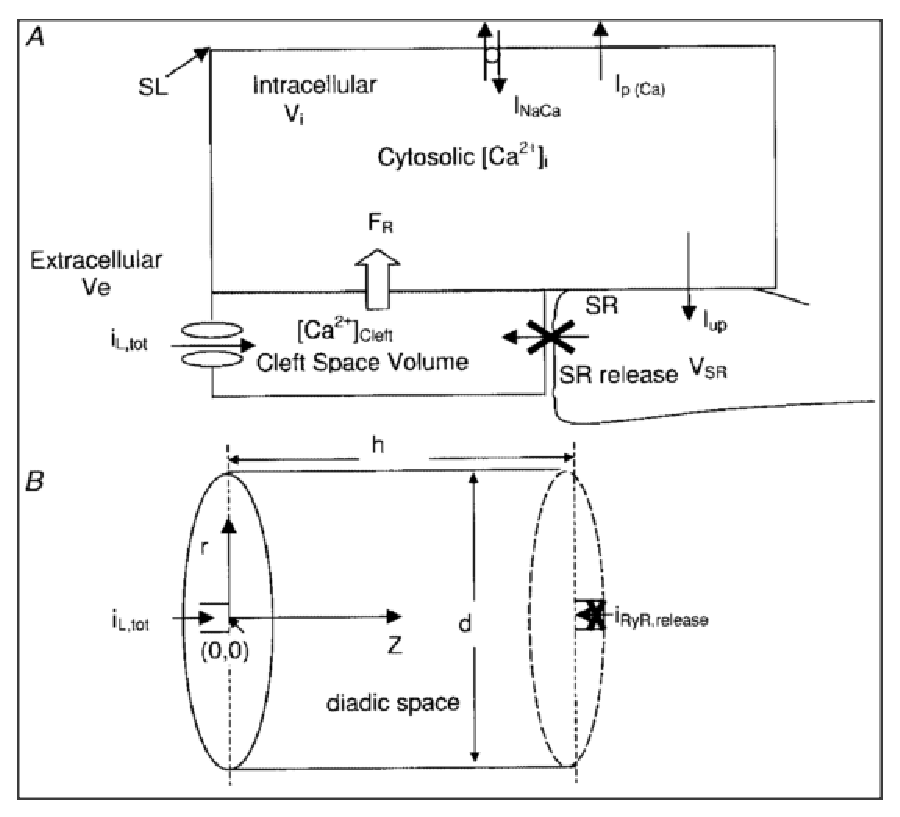
\includegraphics[height=5cm, angle=0]{./images/Sun_cleftspace.eps}}
\caption{Cleft space geometry (only $I_\CaL$ and $I_\ryr$)}
\label{fig:Sun_DHPR_cellmodel}
\end{figure}

Setting: $[\Ca]_o = 1$mM (constant), $\Ca$ ions diffuse passively in the
cylindrical cleft space upon $I_\text{CaL}$ entry.

The model is developed from whole-cell voltage-clamp data. However, single
channel activity was done by averaging the mean open time
\begin{equation}
\bar{t} = \frac{P_o}{r}
\end{equation}
with $r$ is the average opening rate obtained by counting the number of opening
transitions $n$ during the period $T_p$ (the time-averaged current was
calculated). Here, the mean open time increases from 0.84ms at pulse potential
0 mV to 1.7ms at pulse +20 mV. Experimental data: 0.65ms and 1.4ms, respectively
by \citep{fenwick1982}. Other experimental data show $P_o$ increase from nearly
zero at -30mV to 0.6 at +30 mV \citep{reuter1982}.
 
\subsection{Numerical method}

The simulation and analyis were performed on 233MHz Intel PII workstation
running Windows NT 4.0 OS. The parameters involved in GHK equations were found
using a non-linear least-squares method (Marquardt iteration method)
\citep{marquardt1963}. The algorithm was described in \citep{lau1995}
(pp.354-358). The single channel activity simulation was done by embedded the
model into QuB program \citep{qin1996}. 

The numerical method to solve the ODEs was Merson-modified Runge-Kutta 4th-order
adaptive step algorithm \citep{kubicek1983}. The errors from all variables were
normalized to ensure all variables contributed equally to the global error
calculation. 

To solve the diffusion PDE in the cleft space, explicit finite difference scheme
was used, which is similar to that described in \citep{smith1998}.


% \begin{figure}[hbt]
%   \centerline{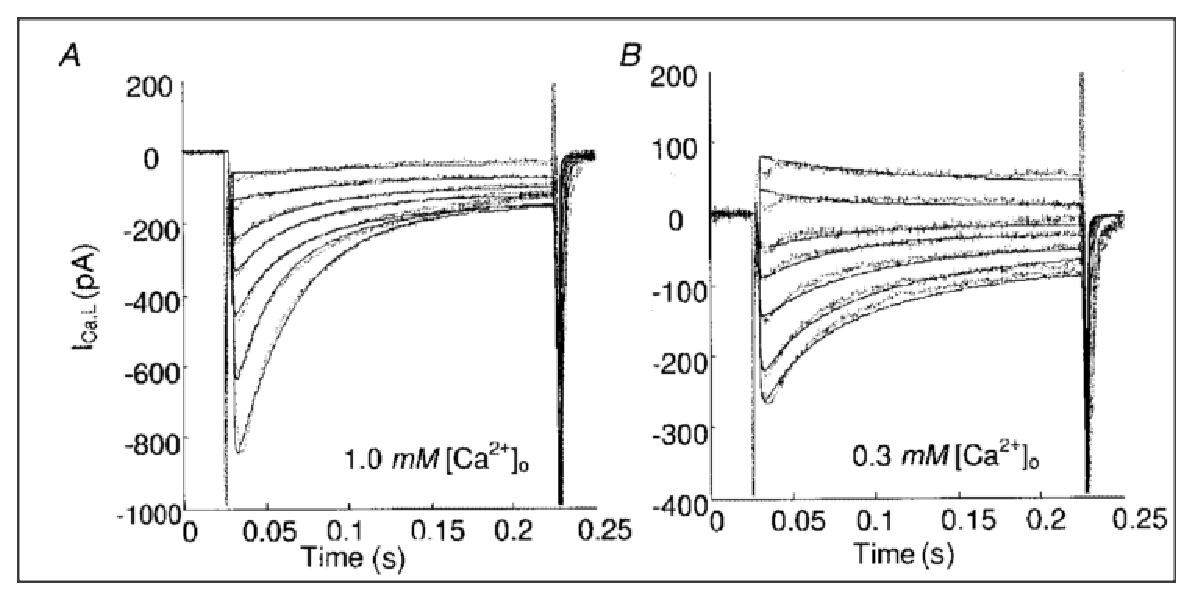
\includegraphics[height=5cm,
%     angle=0]{./images/Sun_experiment_2.eps}}
% \caption{Holding potential -40 mV; labels are extracellular concentration (mM).
% (A) step potential +10mV, (B) +80mV}
% \label{fig:Sun_ICaL}
% \end{figure}


IMPORTANT: Even though the model replicated experimental results, it cannot
produce ``model behavior''. One suggestion is to add one closed state $C_6$ in
front of $C_1$ and utilize a slow rate constant between $\ce{C6 <=> C1}$.


\section{Greenstein-Winslow (2002) - single channel}
\label{sec:LCC_greenstein2002}

\citep{greenstein2002} (Sect.\ref{sec:greenst-winsl-2002}) used a modified version of
mode-switching 12-state LCC model from \citep{jafri1998cad}
(Sect.\ref{sec:LCC_Jafri1998}) and incorporate into a canine ventricular
myocyte model based on \citep{winslow1999} (Sect.\ref{sec:winslow-et-al}). 

Gating of a single L-type $\Ca$ channels (LCC) is modeled using mode-switching
from~\citep{jafri1998cad} (Sect.~\ref{sec:LCC_Jafri1998}) with adjusted
parameters' values.
\begin{itemize}
\item $V_m$-dependent of forward and reverse activation transition
  rate ($\alpha, \beta$) was adjusted based on newer data from canine
  midmyocardial cells \citep{hobai2001}

\item $V_m$-independent transition rate to open states ($f,f'$) are
  adjusted to give peak $P_o$ in the range 5-15\% in response to
  maximal voltage clamp stimulus
  
\item Mode-switching transition rate ($\gamma, \omega$) are adjusted
  to enhance $\Ca$-dependent inactivation.  
  
\item At very positive potential, it can also inactivate the LCC. So,
$V_m$-dependent inactivation of an LCC is incorporated, indicated by $y_{i,j}$
using the simple 2-state gating scheme,  Fig.~\ref{fig:Greenstein_lCC}(B).
Depolarization promotes transition  of some opening channels from the available
state $y$ to the unavailable state  $(1-y)$.

  $V_m$-dependent steady-state inactivation function $y_\infty$ is modified to
  have asymptotic value of 0.6 for large positive membrane.
  \begin{equation}
    \label{eq:1329}
    \begin{split}
        y_\infty &= \frac{0.4}{1+\exp(\frac{V_m+12.5}{5})}+0.6  \\
        \tau_\infty &= \frac{340}{1+e^{(V_m+30)/12}} + 60 \\
        k_{f,y} &= y_\infty/\tau_\infty \\
        k_{b,y} &= \frac{1-y_\infty}{\tau_\infty}
    \end{split}
  \end{equation}
  with $\tau$ in (ms), and $k_{\ldots,y}$ in (ms$^{-1}$).
 
\item $\Ca$ flux via LCC was formulated using GHK equation (constant field
theory). Also, based on local-control theory, the channel senses $[\Ca]$ in
the inner mouth of the channel is $[\Ca]_\ds$, rather than $[\Ca]_\myo$.
 
\item \textcolor{red}{LCC permeability $P_\dhpr$ is adjusted to
  $91.3\mu$m$^3$.s$^{-1}$, which yields a single channel slope
  conductance of 8.2 pS, and unitary current $i_\CaL = \sim -12$pA at 0mV}.
\end{itemize}

\begin{figure}[hbt]
  \centerline{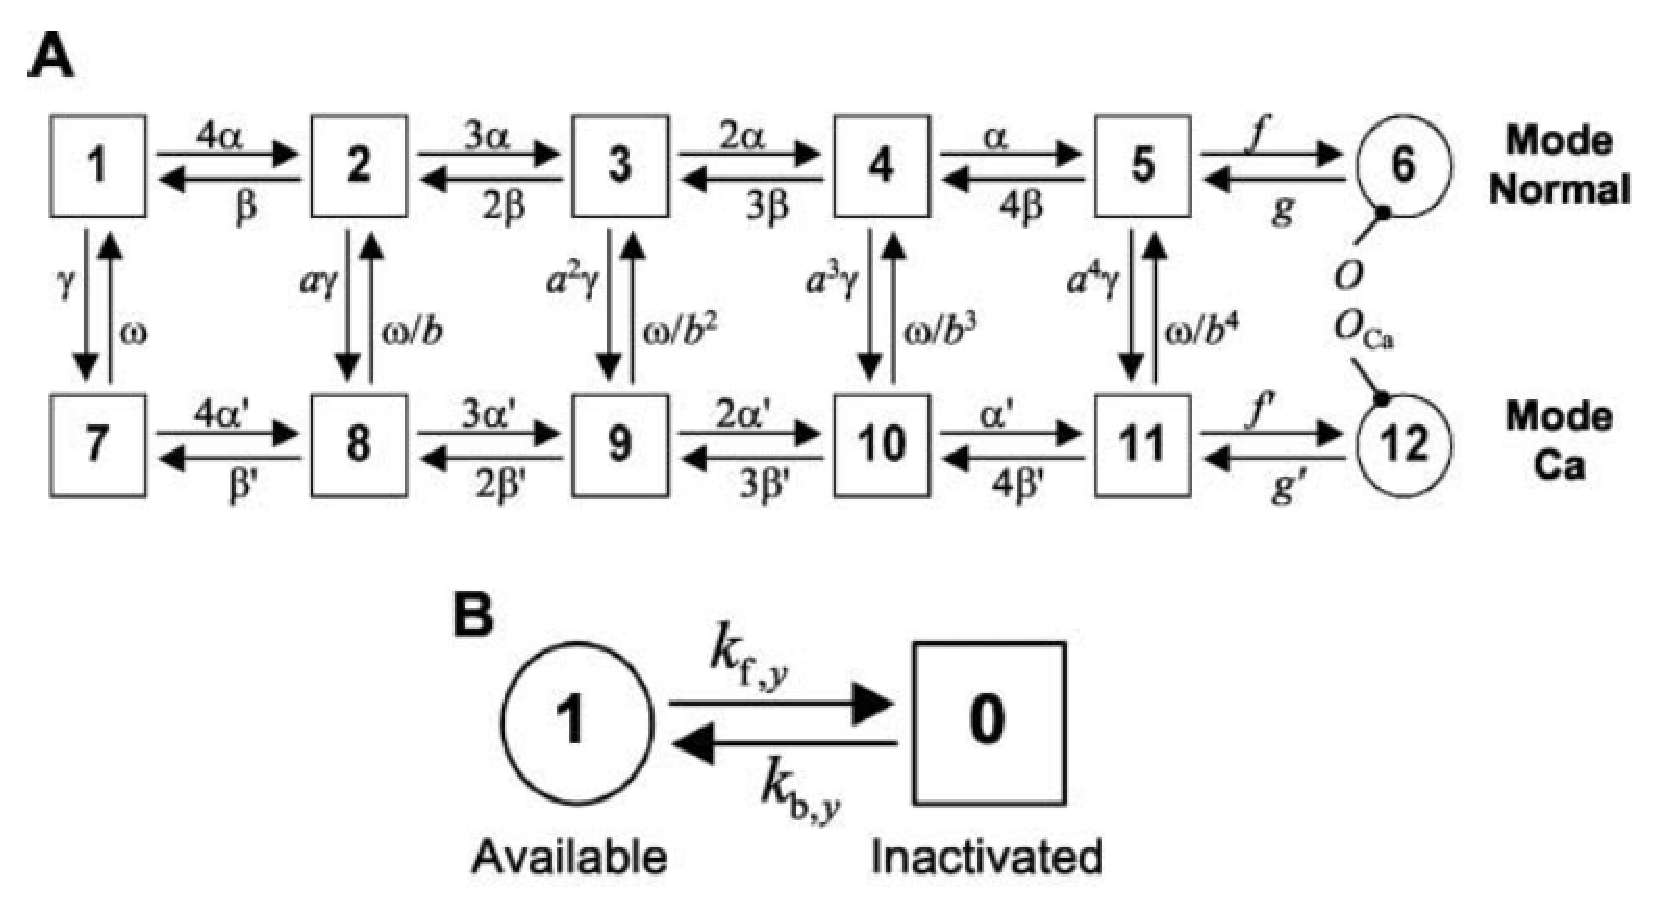
\includegraphics[height=5cm,
    angle=0]{./images/Greenstein_LCC.eps}}
  \caption{(A) Mode-switching of LCC; (B) $V_m$-dependent inactivation
    for LCC}
\label{fig:Greenstein_lCC}
\end{figure}

In the model, the peak current density $I_\CaL \approx 4.7 \muA/$cm$^2$, and a
sustained component of 0.7pA last for nearly the entire duration of AP. The
sustained component is due to LCC keep reopening and $[\Ca]_\ds$ remain
moderately higher than $[\Ca]_\myo$ during AP.

The peak $[\Ca]_\ds$ in the model is about 40$\muM$.
LCC channels open with a dealy 5ms after the triggering. Local jSR release flux
can be triggered by a single LCC opening, and last for $\approx 20$ms. The
longer release gives a high EC gain. The EC gain at 0mV was 12. The mean RyR
open time in the model is $\approx 7$ms. The $\Ca$ sparks (spike) half-maximal
duration in the model was $\approx 25$ms (the experimental value is 20-25ms
using confocal images).

\begin{figure}[hbt]
  \centerline{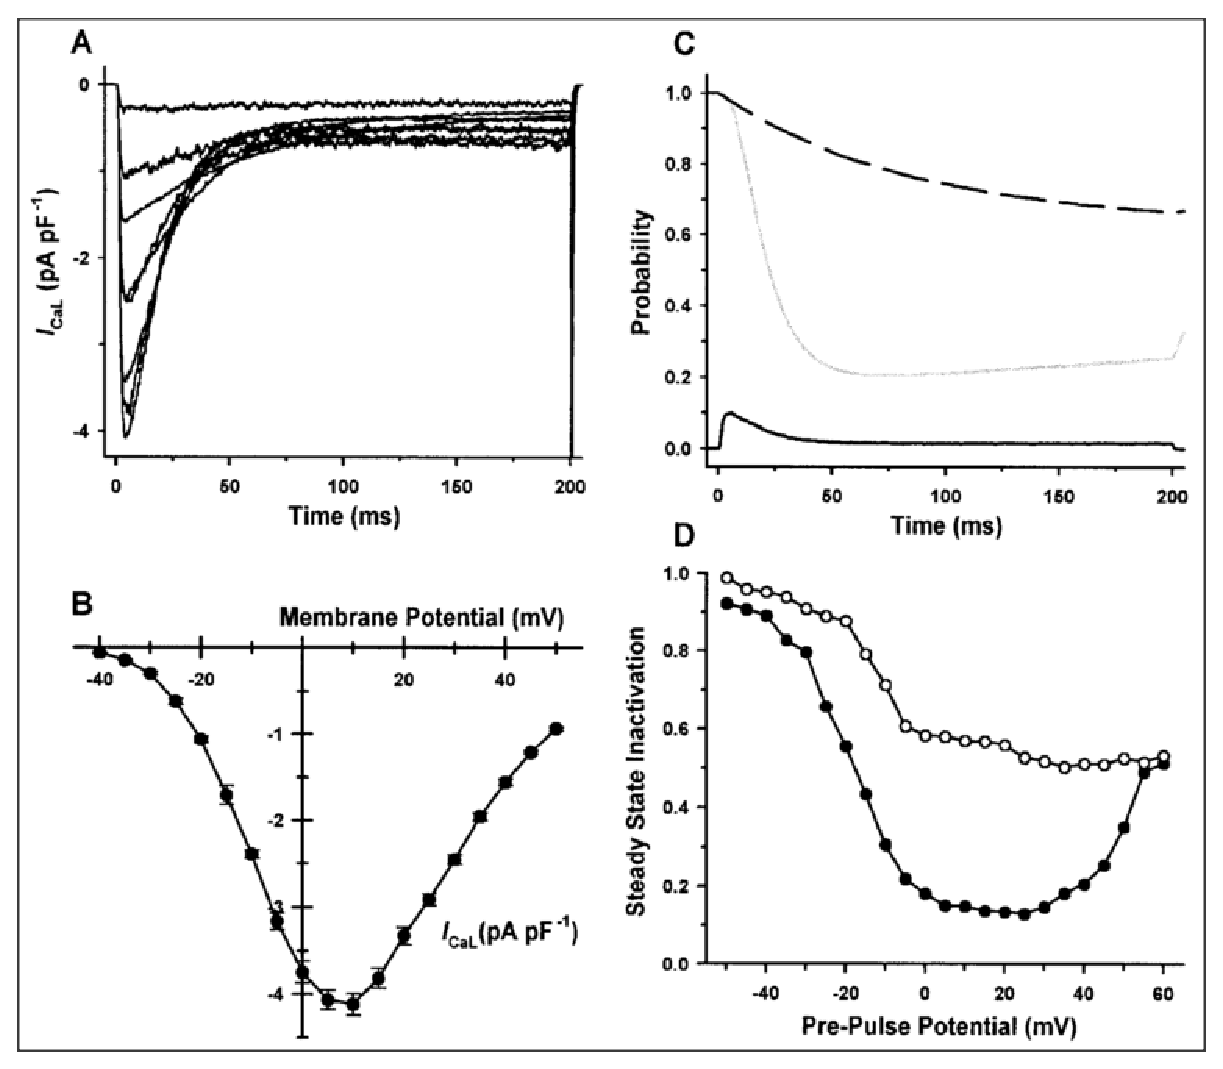
\includegraphics[height=8cm,
    angle=0]{./images/Greenstein_DHPRcurrent.eps}}
  \caption{ (A) macroscopic $I_\CaL$ simulated at different $V_m$ steps (from
  -30mV to +40mV with +10mV increment). (B) mean peak $I_\CaL-V_m$ relation
  averaged from 5 simulation at each potential; (C) $P_o$ of LCC (black solid
  line), and probability that $V_m$-dependent inactivation has not occurred
  (dash line) in response to +0mV step; (D) steady-state inactivation curve
  with (filled circle) and without (open circles) $\Ca$ as charge carrier (we
  can see the effect of $\Ca$ inactivation)}
\label{fig:Greenstein_DHPRcurrent}
\end{figure}

The whole-cell current is given in eq.~\eqref{eq:1218}.
\begin{equation}
  \label{eq:1218}
  I_\CaL = N_\LCC . i_\CaL . p_o . f_\act
\end{equation}
with $N_\LCC$ is the total number of LCC in cells. However, not all of them are
available for conducting, even they're open, until they're phosphorylated
mode.
This phenomenone is incorporated by multiplying with $f_\act$, the fraction of
active channels (i.e. open and is available  for conducting $\Ca$). Finally,
$p_o$ is the open probability for a single channel, and $i_\CaL$ is single channel current.

Typically, the fraction of active channel varies from time to time. However, to
avoid the high computational demand, they made the \textcolor{red}{assumption
that $f_\act$ is constant ($f_\act=0.4$)\citep{handrock1998}, so
  $N_\act=N_\LCC.f_\act$}. So, the new formula for eq.\ref{eq:1218} is
eq.~\eqref{eq:1324}

As $i_\CaL,p_o$ are determined based on experimental constraint for single
channel, $N_\act$ is chosen so that whole-cell $I_\CaL$ reach the whole-cell
measurement in canine~\citep{hobai2001}, i.e. $N_\act=50,000$ which
corresponds to \textcolor{red}{$N_\CRU = 12,500$ CRUs}.





\section{Koh-\ldots-Levchenko (2006) - human (single channel)}
\label{sec:LCC_Koh2006}

In previous LCC models, the $\Ca$-dependent inactivation is derived from
$[\Ca]_\ds$. However, the underlying mechanism is that calcium ions bind to
CaM and $\Ca$/CaM complex that inactivate the channel. \citep{koh2006} developed
an LCC model that account for the binding kinetics of individual $\Ca$ ions to
CaM. Here, they assume the high-affinity sites, but not the low-affinity sites,
are responsible for the inactivation process \citep{peterson1999}. So, binding
of two $\Ca$ ions at the two high-affinity sites is enough for triggering the
inactivation.

Here, the binding of $\Ca$ to Calmodulin is assumed to occur regardless whether
the channel is opening or not. As shown in Fig.\ref{fig:LCC_Koh2003}, LCC enters
$\Ca$-inactivated states after two $\Ca$-binding events at the high-affinity
$\CaM$ sites, Fig.\ref{fig:LCC_Koh2003}. Here, the recovery from $\Ca$-dependent
inactivation is governed by the dissociation of $\Ca$ from $\Ca$/CaM complex.

To account for the voltage-dependent inactivation, they assume from any of the 6
states, it can switch to voltage-inactivation state; and this process is
irreversible during the simulation of 250 ms.  \citep{koh2006} used this
mode-switching model in their stochastic  Monte-Carlo simulation of $\Ca$ sparks
(Sect.\ref{sec:koh_levchenko_2006}). 

\begin{figure}[hbt]
  \centerline{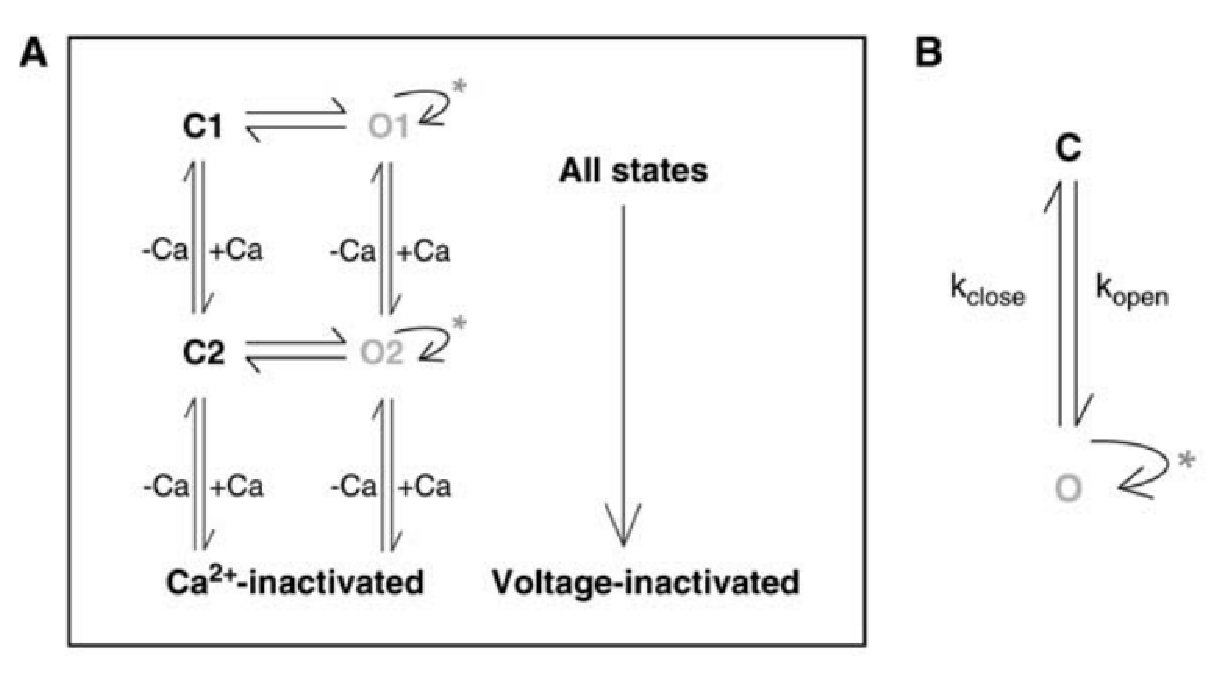
\includegraphics[height=5cm,
    angle=0]{./images/LCC_Koh2003.eps}}
  \caption{The generation of $\Ca$ is indicated by {\it asterisks} transitions
  at the Open states. 
  }
\label{fig:LCC_Koh2003}
\end{figure}


\subsection{Parameter estimation}

To model the effect of non-phosphorylated and phoshorylated LCC models, they
used the same scheme, yet with different reaction parameters obtained from
\citep{schroder1998}.

Rate constants (unit: s$^{-1}$) are derived from a study on single LCC
availability and $P_o$ in healthy and failing human ventricles
\citep{schroder1998}. The unitary current (unit: pA) is represented in terms of
the rate of $\Ca$ entry (unit: s$^{-1}$). The list of rate constants is given
in Table \ref{tab:LCC_Koh2006}. 

Experimental data: \citep{wang2001,findlay2002,Johnson1996,schroder1998}.	

\begin{table}[hbt]
\begin{tabular}{cc}
$k_\text{O1-O1} = 10^6 [\text{s}^{-1}]$ & \citep{wang2001} \\
$k_\text{O2-O2} =  $ & at 0mV, 23-25$^\circ$C, rat ventricular myocyte \\
$k_\text{C1-C2} = 2.3 [1/(\muM.s)]$ & \\
$k_\text{O1-O2} = 2.4 [s^{-1}] $ & \\
\ldots & \ldots 
\end{tabular}
\label{tab:LCC_Koh2006}
\caption{Parameters}
\end{table}



\section{Bondarenko et al. (2004) - ferret}
\label{sec:LCC_Bondarenko2004}

\citep{bondarenko2004mgc,bondarenko2004cma} developed 8-state Markov-based model
for ferret ventricular myocyte, Fig.\ref{fig:LCCmodel_Bondarenko2004}.
There are 4 closed states (C$_1$-C$_4$), one open state (O), and three activate
state (I$_1$-I$_3$).

\begin{figure}[hbt]
  \centerline{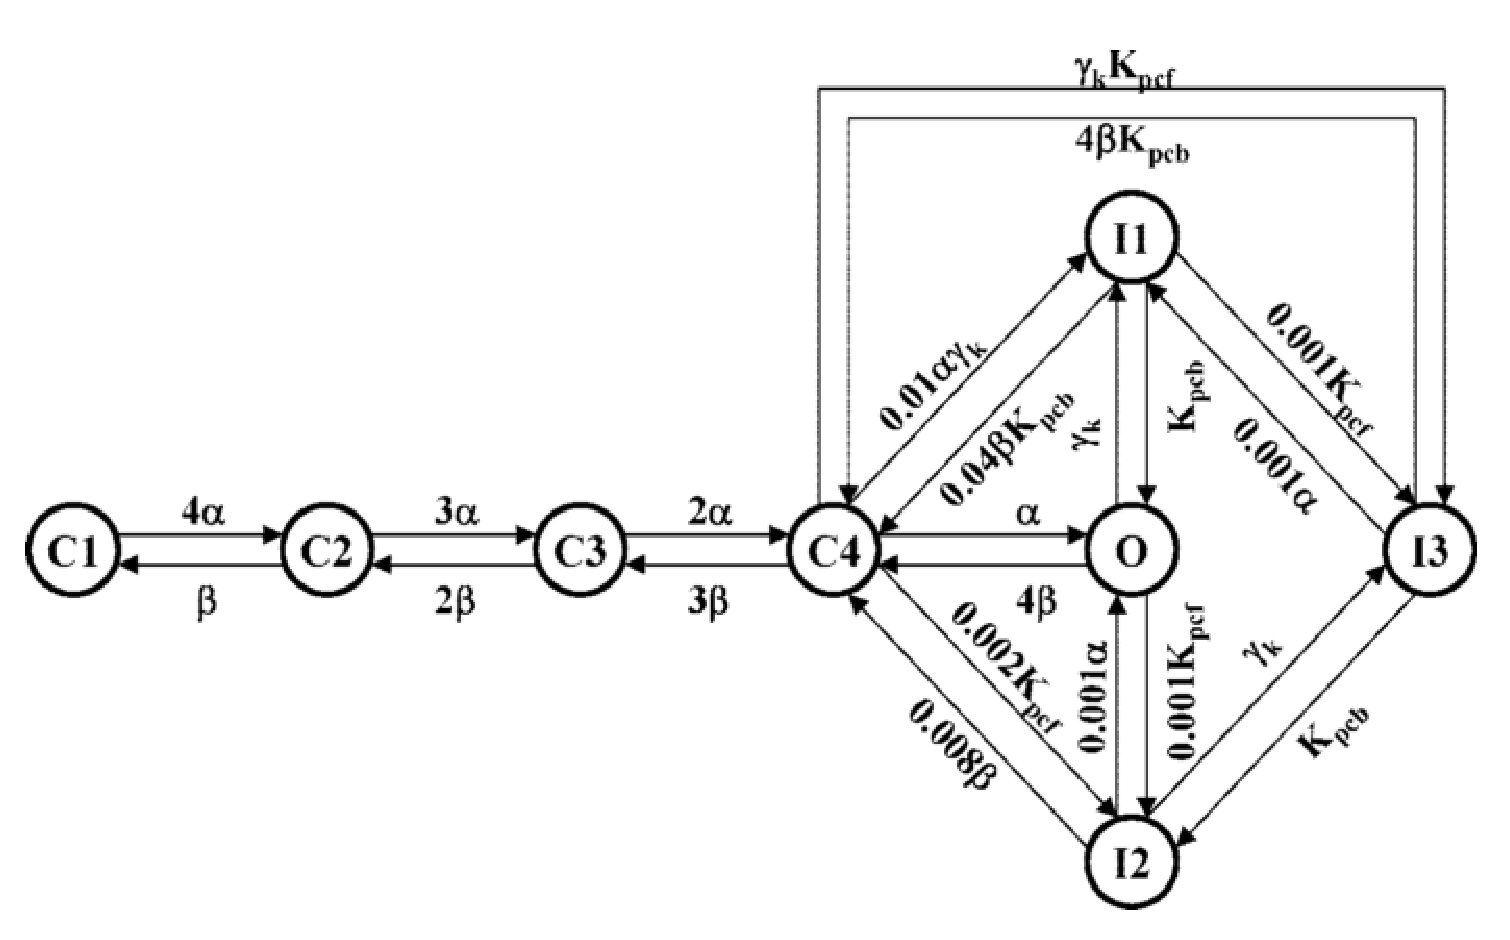
\includegraphics[height=6cm,
    angle=0]{./images/LCCmodel_Bondarenko2004.eps}}
\caption{A 8-state model of L-type $\Ca$ channel}
\label{fig:LCCmodel_Bondarenko2004}
\end{figure}


\section{Hinch et al. (2004)}

\citep{hinch2004slc} 

\section{Faber-Rudy (2007)}
\label{sec:LCC_Faber2007}

\citep{faber2007DHPR} studied missense mutation G406R that causes Timothy
syndrome which is characterized by a prolonged QT interval on the ECG and
arrhythmia development, and many other organ dysfunctions.

Here, the global cellular approach is used where only a single subsarcolemmal
space, along the length of the T-tubules, into where calcium from L-type $\Ca$
channels and RyR flows. IMPORTANT: This approach is not suitable to simulate
local microscopic processes of $\Ca$ sparks. 

The 14-state model that mirrors two mode: mode voltage and mode calcium,
Fig.\ref{fig:LCC_Faber2007}. There is only one conducting state. It's assumed
four voltage sensitivie transitions before the channel opening to reflect the 4
voltage sensors, each in each homologous domains making up the
$\alpha_\text{1C}$ and to describe the complex channel behavior (fast and slow
voltage-dependent). The model is based on the assumption that the channel can be
inactivated by calcium at any time, regardless of whether the channel is opening
or not.

\begin{figure}[hbt]
  \centerline{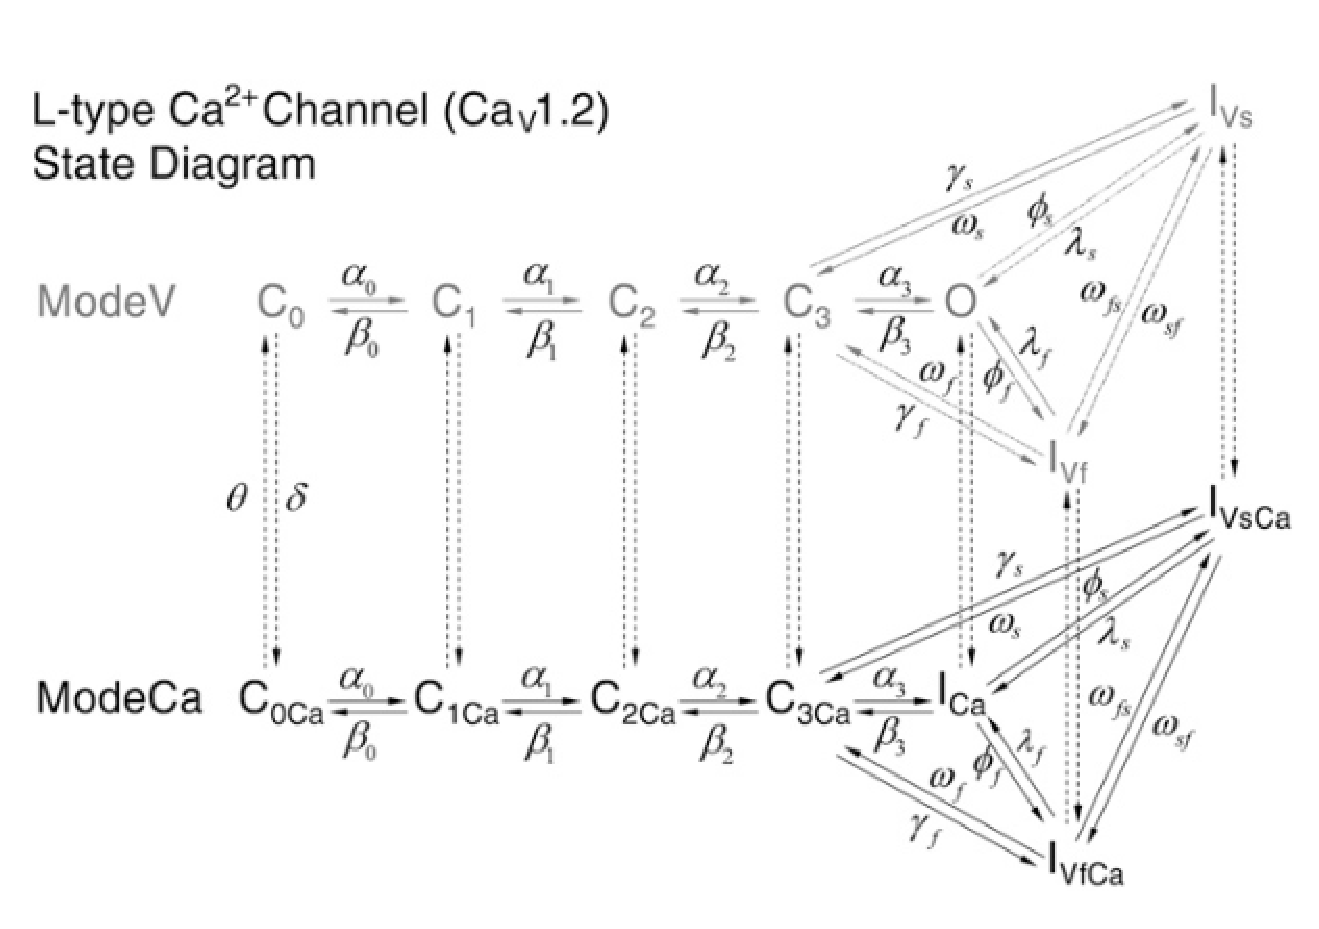
\includegraphics[height=4cm,
    angle=0]{./images/LCC_Faber2007.eps}}
\caption{LCC Markov model. The upper tier (mode $V_m$) represents the
voltage-dependent inactivation and the lower tier (ModeCa) represent
$Ca$-dependent inactivation}
\label{fig:LCC_Faber2007}
\end{figure}

To estimate the parameters for the model, using experimental data that doesn't
use $\Ca$ as the charge carriers, then the transition rates from Mode V to
ModeCa are all set to zero. The model was then validated using experimental data
from guinea pig ventricular myocytes at 37$^\circ$C. Also, the data were
recorded without $\beta$-agonists as they have found to significantly effect on
current magnitude, voltage-dependent properties, and $\Ca$-dependent properties
of the channels.



\subsection{Case studies}

In Timothy syndrome, the VDI pathway is eliminated while leaving the CDI
unaffected \citep{splawski2004, splawski2005}. 

\section{Mahajan et al. (2008)}
\label{sec:LCC_Mahajan2008}

\citep{mahajan2008} (Sect.\ref{sec:mahajan_weiss_2008}) proposed a new LCC
model.  The model was developed using data from rabbit ventricular myocytes and
applied to \citep{shannon2004} rabbit ventricular AP model
(Sect.\ref{sec:shannon_2004_rabbit}).

The 7-state model, Fig.\ref{fig:LCC_Mahajan08}, was developed using patch-clamp
data at 35-37$^\circ$C, which has both CDI and VDI. Macroscopic currents were
recorded using voltage- or current-clamp conditions for whole-cell, technique
described in \citep{rae1991}. 

The current traces of experimental data at -20, -10, 0, +10, +20 and +30 mV were
used to fit the parameters. The multi parameters were fit using multidimensional
least squares algorithm from Berekeley Madonna software package. Microscopic
reversibility was implemented for all closed loops.

\subsection{VDI}

Voltage-depenent activation (VDA) controls the transition between closed states.
A detailed model uses 4 closed states (representing the gating each of the 4
subunits). Here, they choose to use only 2 closed states, with the transition
from C2 to C1 is strongly voltage-dependent.

\begin{figure}[hbt]
  \centerline{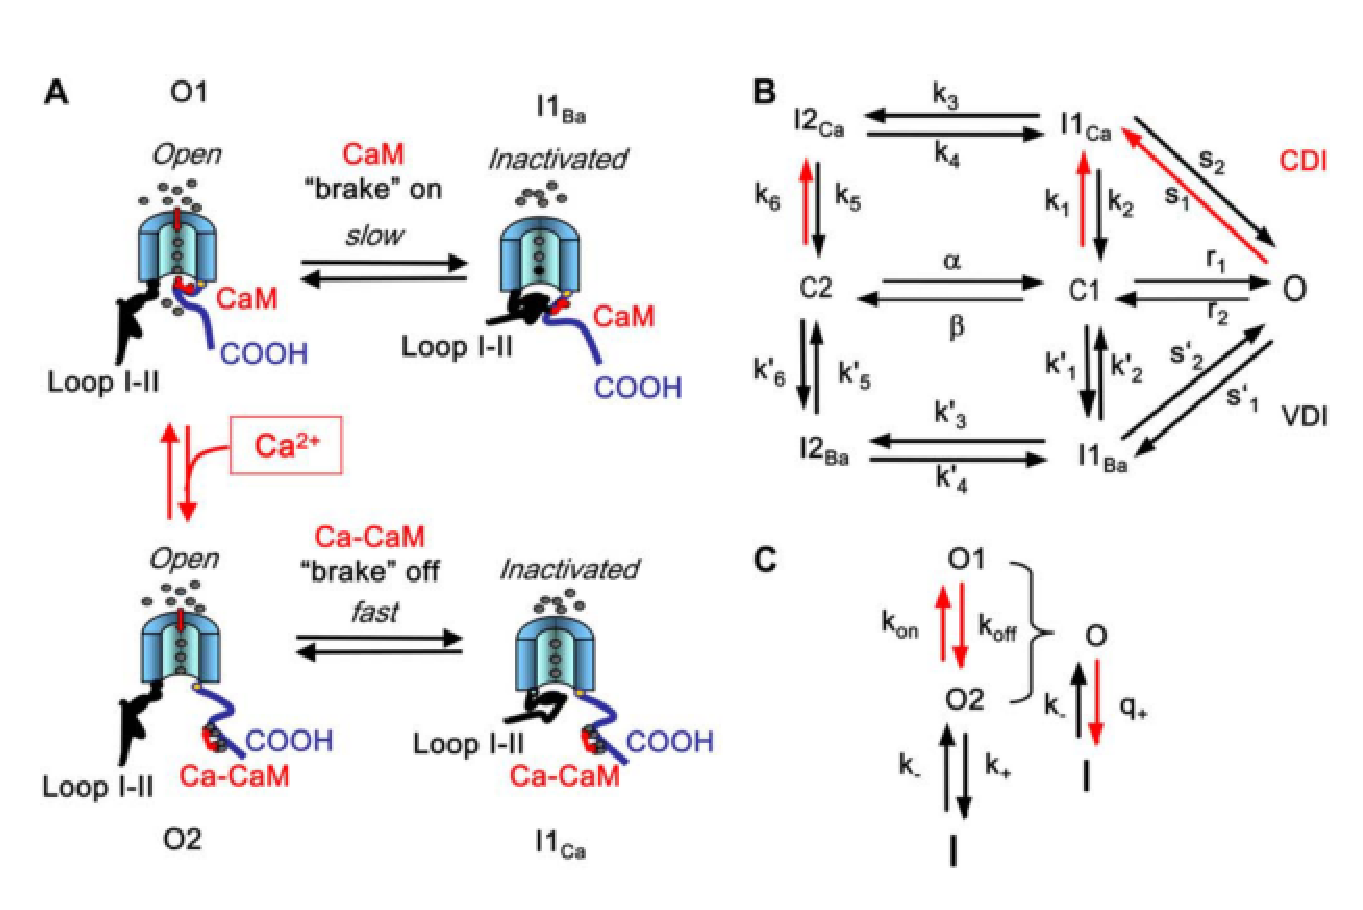
\includegraphics[height=7cm,
    angle=0]{./images/LCC_Mahajan08.eps}}
  \caption{7-state model}
  \label{fig:LCC_Mahajan08}
\end{figure}

The transition from C1 to open O is voltage-independent and determine the
steady-state open probability.





\section[Hashambhoy-Winslow-Greenstein (2009)]{Hashambhoy-Winslow-Greenstein
(2009) - CaMKII (canine)}
\label{sec:LCC_CaMKII_Hashambhoy2009}



Typically, LCC is modeled with 2 modes. Mode 1 is the dominant form of LCC
gating, characterized by repeated brief opening. Mode 2 is the high-activity
gating mode, characterized by prolonged channel openings. 
Inhibition of CaMKII activity significantly decreases the likelihood of early
afterdepolarization (EAD) in rabbit hearts \citep{Dzhura2000}. The functional
result of CaMKII-mediatd events is $I_\CaL$ facilitation, i.e. increasing channel open
probability \citep{}. This can be explained by different hypothesis:
\begin{enumerate}
  \item an increase rate of recovery from $\Ca$-dependent inactivation (CDI).
  \item a shift to high-activity gating mode
\end{enumerate} 
The structure and functions of CaMKII has been studied under different
conditions. From that, different multi-state CaMKII models have been proposed,
as functions of $\Ca$ and calmodulin concentration\citep{Kubota2001,Dupont2003}.
Hashambhoy et al. model is based on CaMKII model by \citep{Dupont2003}, and
assumed the second hypothesis, i.e. shift in gating-mode.
The hypothesis was tested by incorporating into the canine model by
\citep{greenstein2002}. \textcolor{red}{The result suggests that the shift in
gating mode is enough to account for increased $I_\CaL$ amplitude.}

Here, each CaMKII holoenzyme is tethered to a single LCC. The states of the
CaMKII will determine the state of LCC. 
\begin{enumerate}
  \item \citep{Dupont2003} developed a 5-state
deterministic model for CaMKII. Hashambhoy et al. add 2 new states: 

The transitions between states are controled by $\Ca$ levels, CaM, phosphatase,
and the activity of neighboring CaMKII subunits in the same holoenzyme. Here,
they restrict autophosphorylation events to
occur between adjacent CaMKII  subunits. 
   
\end{enumerate}


The LCC model is mode-switching 12-state based on \citep{greenstein2002} with
the only difference in the channel closing parameter $g$ and $g'=$.  




%%% Local Variables: 
%%% mode: latex
%%% TeX-master: "mainfile"
%%% End: 
